% This example is meant to be compiled with lualatex or xelatex
% The theme itself also supports pdflatex
\PassOptionsToPackage{unicode}{hyperref}
\documentclass[aspectratio=1610, xcolor=dvipsnames, 9pt]{beamer}

% Load packages you need here
\usepackage{polyglossia}
\setmainlanguage{german}

\usepackage{csquotes}
\usepackage{smartdiagram}

\usepackage{amsmath}
\usepackage{amssymb}
\usepackage{mathtools}

\usepackage{hyperref}
\usepackage{bookmark}

% load the theme after all packages

\usetheme[
  showtotalframes, % show total number of frames in the footline
]{fhswf}

% Put settings here, like
\unimathsetup{
  math-style=ISO,
  bold-style=ISO,
  nabla=upright,
  partial=upright,
  mathrm=sym,
}

\title{Neuronale Netze/Deep Learning und Predictive Maintenance}
\author[F.~Neubürger,]{ \textbf{Felix Neubürger}}
\institute[I \& W]{Fachhochschule Südwestfalen, Ingenieurs- \& Wirtschaftswissenschaften}
\date{01. Oktober 2025}
\titlegraphic{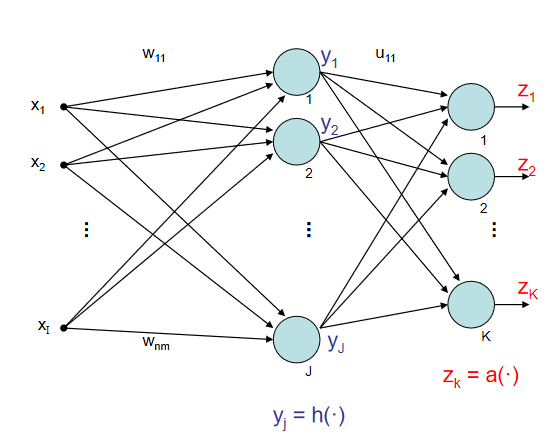
\includegraphics[width=0.2\textwidth]{images/MLP2.png}}


\begin{document}


\begin{frame}{Inhalte der Vorlesung}
  \begin{columns}
    \begin{column}{1\textwidth}
      \begin{itemize}
        \item Wiederholung Neuronale Netze (NN)\newline
        \item Einführung spezieller Architekturen Neuronaler Netze \newline
        \item Anwendung von Neuronalen Netzen zur Lösung zur Datenanalyse  \newline
        \item Verschiedene Architekturen Neuronaler Netze \newline 
      \end{itemize}
    \end{column}
    \begin{column}{0\textwidth}
% \begin{figure}
% \centering
%             \includegraphics[width=0.9\textwidth]{images/intro/intro.pdf}
% \end{figure}
    \end{column}
  \end{columns}
\end{frame}

\begin{frame}{Ziele der Vorlesung - Welche Fragen sollen beantwortet werden?}
  \begin{columns}
    \begin{column}{0.69\textwidth}
      \begin{itemize}
        \item Was genau machen Neuronale Netze? \newline
        \item Wie kann ich mir das vorstellen? \newline
        \item Was ist überhaupt "Deep Learning"?  \newline
        \item Welche verschiedenen Architekturen neuronaler Netze gibt es? \newline
        \item Muss es immer Deep Learning sein? \newline
      \end{itemize}
    \end{column}
    \begin{column}{0.3\textwidth}
 \begin{figure}
 \centering
             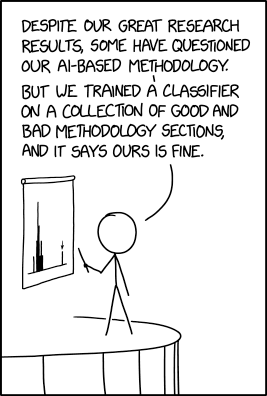
\includegraphics[width=0.9\textwidth]{images/ai_methodology.png}
             [\url{https://xkcd.com/2451/}]
 \end{figure}
    \end{column}
  \end{columns}
\end{frame}

\begin{frame}{Mathematischer Refresher -- Vektoren und Matrizen}
  \begin{columns}
    \begin{column}{1\textwidth}
      \begin{itemize}
        \item \textbf{Vektor}: Spaltenvektor $\mathbf{x} \in \mathbb{R}^d$ mit $d$ Komponenten
        \begin{equation}
          \mathbf{x} = \begin{pmatrix} x_1 \\\\ x_2 \\\\ \vdots \\\\ x_d \end{pmatrix}
        \end{equation}
        \item \textbf{Zeilenvektor}: $\mathbf{x}^T = (x_1, x_2, \ldots, x_d)$ (Transponiert)
        \item \textbf{Matrix}: $\mathbf{A} \in \mathbb{R}^{m \times n}$ mit $m$ Zeilen und $n$ Spalten
        \begin{equation}
          \mathbf{A} = \begin{pmatrix}
            a_{11} & a_{12} & \cdots & a_{1n} \\\\
            a_{21} & a_{22} & \cdots & a_{2n} \\\\
            \vdots & \vdots & \ddots & \vdots \\\\
            a_{m1} & a_{m2} & \cdots & a_{mn}
          \end{pmatrix}
        \end{equation}
        \item \textbf{Indexierung}: $a_{ij}$ = Element in Zeile $i$, Spalte $j$
      \end{itemize}
    \end{column}
  \end{columns}
\end{frame}

\begin{frame}{Mathematischer Refresher -- Grundoperationen}
  \begin{columns}
    \begin{column}{1\textwidth}
      \begin{itemize}
        \item \textbf{Skalarprodukt} (Dot Product): Für $\mathbf{x}, \mathbf{y} \in \mathbb{R}^d$
        \begin{equation}
          \mathbf{x}^T \mathbf{y} = \mathbf{x} \cdot \mathbf{y} = \sum_{i=1}^{d} x_i y_i
        \end{equation}
        \item \textbf{Matrix-Vektor-Multiplikation}: $\mathbf{A} \in \mathbb{R}^{m \times n}, \mathbf{x} \in \mathbb{R}^n$
        \begin{equation}
          \mathbf{y} = \mathbf{A}\mathbf{x} \in \mathbb{R}^m, \quad y_i = \sum_{j=1}^{n} a_{ij} x_j
        \end{equation}
        \item \textbf{Matrix-Matrix-Multiplikation}: $\mathbf{A} \in \mathbb{R}^{m \times k}, \mathbf{B} \in \mathbb{R}^{k \times n}$
        \begin{equation}
          \mathbf{C} = \mathbf{A}\mathbf{B} \in \mathbb{R}^{m \times n}, \quad c_{ij} = \sum_{\ell=1}^{k} a_{i\ell} b_{\ell j}
        \end{equation}
        \item \textbf{Elementweise Operationen}: Hadamard-Produkt $\mathbf{A} \odot \mathbf{B}$
        \begin{equation}
          (\mathbf{A} \odot \mathbf{B})_{ij} = a_{ij} \cdot b_{ij}
        \end{equation}
      \end{itemize}
    \end{column}
  \end{columns}
\end{frame}

\begin{frame}{Mathematischer Refresher -- Normen und Abstände}
  \begin{columns}
    \begin{column}{1\textwidth}
      \begin{itemize}
        \item \textbf{Euklidische Norm}: $||\mathbf{x}||_2 = \sqrt{\sum_{i=1}^{d} x_i^2}$ (Länge des Vektors)
        \item \textbf{L1-Norm}: $||\mathbf{x}||_1 = \sum_{i=1}^{d} |x_i|$ (Manhattan-Distanz)
        \item \textbf{Unendlich-Norm}: $||\mathbf{x}||_\infty = \max_i |x_i|$ (Maximum-Norm)
        \item \textbf{Frobenius-Norm} (für Matrizen): $||\mathbf{A}||_F = \sqrt{\sum_{i,j} a_{ij}^2}$
        \item \textbf{Einheitsvektor}: $\mathbf{u}$ mit $||\mathbf{u}||_2 = 1$
        \item \textbf{Orthogonale Vektoren}: $\mathbf{x} \perp \mathbf{y}$ wenn $\mathbf{x}^T \mathbf{y} = 0$
        \item \textbf{Linearkombination}: $\mathbf{y} = \alpha_1 \mathbf{x}_1 + \alpha_2 \mathbf{x}_2 + \ldots + \alpha_k \mathbf{x}_k$
      \end{itemize}
    \end{column}
  \end{columns}
\end{frame}

\begin{frame}{Mathematischer Refresher -- Differentiation und Gradienten}
  \begin{columns}
    \begin{column}{1\textwidth}
      \begin{itemize}
        \item \textbf{Partielle Ableitung}: Für $f: \mathbb{R}^n \to \mathbb{R}$
        \begin{equation}
          \frac{\partial f}{\partial x_i} = \lim_{h \to 0} \frac{f(\mathbf{x} + h\mathbf{e}_i) - f(\mathbf{x})}{h}
        \end{equation}
        \item \textbf{Gradient}: Vektor aller partiellen Ableitungen
        \begin{equation}
          \nabla f(\mathbf{x}) = \begin{pmatrix}
            \frac{\partial f}{\partial x_1} \\\\
            \frac{\partial f}{\partial x_2} \\\\
            \vdots \\\\
            \frac{\partial f}{\partial x_n}
          \end{pmatrix}
        \end{equation}
        \item \textbf{Kettenregel}: Für $f(g(x))$
        \begin{equation}
          \frac{d}{dx} f(g(x)) = f'(g(x)) \cdot g'(x)
        \end{equation}
        \item \textbf{Multivariable Kettenregel}: Für $f(\mathbf{u}(\mathbf{x}))$
        \begin{equation}
          \frac{\partial f}{\partial x_i} = \sum_j \frac{\partial f}{\partial u_j} \frac{\partial u_j}{\partial x_i} = \nabla_\mathbf{u} f \cdot \frac{\partial \mathbf{u}}{\partial x_i}
        \end{equation}
      \end{itemize}
    \end{column}
  \end{columns}
\end{frame}

\begin{frame}{Mathematischer Refresher -- Wichtige Funktionen und Eigenschaften}
  \begin{columns}
    \begin{column}{1\textwidth}
      \begin{itemize}
        \item \textbf{Exponentialfunktion}: $e^x$, Ableitung: $\frac{d}{dx} e^x = e^x$
        \item \textbf{Logarithmus}: $\ln(x)$, Ableitung: $\frac{d}{dx} \ln(x) = \frac{1}{x}$
        \item \textbf{Sigmoid-Funktion}: $\sigma(x) = \frac{1}{1 + e^{-x}}$
        \begin{equation}
          \sigma'(x) = \sigma(x)(1 - \sigma(x))
        \end{equation}
        \item \textbf{Quadratische Funktion}: $f(x) = ax^2 + bx + c$, Ableitung: $f'(x) = 2ax + b$
        \item \textbf{Produktregel}: $(fg)' = f'g + fg'$
        \item \textbf{Summenregel}: $(f + g)' = f' + g'$
        \item \textbf{Konstante Faktoren}: $(cf)' = cf'$ für Konstante $c$
      \end{itemize}
    \end{column}
  \end{columns}
\end{frame}

\begin{frame}{Mathematische Notation -- Überblick für diese Vorlesung}
  \begin{columns}
    \begin{column}{1\textwidth}
      \begin{itemize}
        \item \textbf{Skalare}: Kleinbuchstaben $a, b, c, x, y, z$
        \item \textbf{Vektoren}: Fettgedruckte Kleinbuchstaben $\mathbf{x}, \mathbf{y}, \mathbf{w}, \mathbf{b}$
        \item \textbf{Matrizen}: Fettgedruckte Großbuchstaben $\mathbf{A}, \mathbf{W}, \mathbf{X}$
        \item \textbf{Mengen}: Kalligrafische Buchstaben $\mathcal{D}, \mathcal{M}, \mathcal{X}$
        \item \textbf{Funktionen}: $f, g, h, L$ (Verlustfunktion)
        \item \textbf{Aktivierungsfunktionen}: $\sigma, \text{ReLU}, \tanh$
        \item \textbf{Indizes}:
        \begin{itemize}
          \item $i, j, k$: Datenindizes, Neuron-Indizes
          \item $(\ell)$: Schicht-Index, z.B. $\mathbf{W}^{(\ell)}$
          \item $(t)$: Zeit-/Iterationsindex, z.B. $\mathbf{w}^{(t)}$
        \end{itemize}
        \item \textbf{Wahrscheinlichkeiten}: $P, p, \mathbb{E}[\cdot]$ (Erwartungswert)
        \item \textbf{Approximation}: $\approx$, Proportionalität: $\propto$
      \end{itemize}
    \end{column}
  \end{columns}
\end{frame}


  \begin{frame}{Was sind Neuronale Netze und was ist Deep Learning?}
        \begin{columns}
          \begin{column}{0.7\textwidth}
            \begin{itemize}
              \item Abstrakt: Verkettung nichtlinearer Abbildungen \newline
              \item Die Parameter dieser Abbildungen wird mit vorhandenen Daten "gelernt" \newline
              \item Verschiedene Optimierungsverfahren zur Festlegung der "besten" Parameter \newline
            \end{itemize}
          \end{column}
          \begin{column}{0.3\textwidth}
       \begin{figure}
       \centering
                   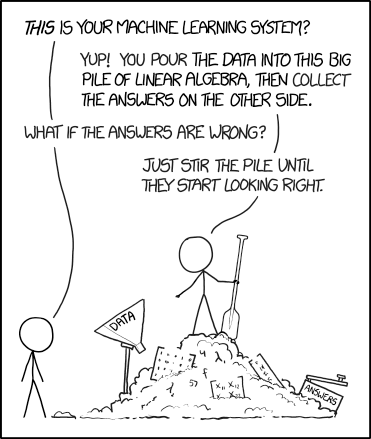
\includegraphics[width=0.9\textwidth]{images/machine_learning.png}\newline
             [\url{https://xkcd.com/1838/}]
       \end{figure}
          \end{column}
        \end{columns}
      \end{frame}

\begin{frame}{Warum funktionieren Neuronale Netze? -- Mathematische Intuition}
  \begin{columns}
    \begin{column}{1\textwidth}
      \begin{itemize}
        \item \textbf{Grundproblem}: Finde eine Funktion $f: \mathbb{R}^d \to \mathbb{R}^k$, die Eingaben $\mathbf{x}$ auf gewünschte Ausgaben $\mathbf{y}$ abbildet
        \item \textbf{Funktionsapproximation}: Neuronale Netze sind universelle Funktionsapproximatoren
        \item \textbf{Komposition einfacher Funktionen}: 
        \begin{equation}
          f(\mathbf{x}) = f_L \circ f_{L-1} \circ \ldots \circ f_2 \circ f_1(\mathbf{x})
        \end{equation}
        \item Jede Schicht $f_i$ führt eine \textbf{affine Transformation} gefolgt von \textbf{Nichtlinearität} aus:
        \begin{equation}
          f_i(\mathbf{x}) = \sigma_i(\mathbf{W}_i \mathbf{x} + \mathbf{b}_i)
        \end{equation}
        \item \textbf{Warum Nichtlinearität wichtig ist}: Ohne sie wäre das gesamte Netz nur eine lineare Transformation
        \begin{equation}
          \mathbf{W}_L(\mathbf{W}_{L-1}(\ldots(\mathbf{W}_1 \mathbf{x}))) = (\mathbf{W}_L \mathbf{W}_{L-1} \ldots \mathbf{W}_1) \mathbf{x} = \mathbf{W}_{\text{eff}} \mathbf{x}
        \end{equation}
      \end{itemize}
    \end{column}
  \end{columns}
\end{frame}

\begin{frame}{Warum funktionieren Neuronale Netze? -- Universal Approximation Theorem}
  \begin{columns}
    \begin{column}{1\textwidth}
      \begin{itemize}
        \item \textbf{Universal Approximation Theorem} \cite{cybenko1989,hornik1991}:
        \item Ein Feedforward-Netz mit einer versteckten Schicht kann jede stetige Funktion auf einem kompakten Definitionsbereich beliebig genau approximieren
        \item \textbf{Mathematische Formulierung}: Sei $\sigma: \mathbb{R} \to \mathbb{R}$ eine nicht-konstante, beschränkte und monotone Aktivierungsfunktion. Dann kann für jede stetige Funktion $g: [0,1]^d \to \mathbb{R}$ und $\epsilon > 0$ eine Funktion
        \begin{equation}
          F(\mathbf{x}) = \sum_{i=1}^N \alpha_i \sigma(\mathbf{w}_i^T \mathbf{x} + b_i)
        \end{equation}
        gefunden werden, sodass $|F(\mathbf{x}) - g(\mathbf{x})| < \epsilon$ für alle $\mathbf{x} \in [0,1]^d$
        \item \textbf{Praktische Bedeutung}: 
        \begin{itemize}
          \item Theoretisch können neuronale Netze jede Funktion lernen
          \item Problem: Anzahl der benötigten Neuronen kann exponentiell wachsen
          \item Deep Learning: Mehr Schichten können effizienter sein als breitere Netze
        \end{itemize}
      \end{itemize}
    \end{column}
  \end{columns}
\end{frame}

\begin{frame}{Die Mathematik des Lernens -- Warum Gradientenabstieg funktioniert}
  \begin{columns}
    \begin{column}{1\textwidth}
      \begin{itemize}
        \item \textbf{Optimierungsproblem}: Minimiere Verlustfunktion $L(\boldsymbol{\theta})$ über Parameter $\boldsymbol{\theta}$
        \item \textbf{Gradientenabstieg basiert auf Taylor-Entwicklung}:
        \begin{equation}
          L(\boldsymbol{\theta} + \boldsymbol{\Delta\theta}) \approx L(\boldsymbol{\theta}) + \nabla L(\boldsymbol{\theta})^T \boldsymbol{\Delta\theta}
        \end{equation}
        \item Um $L$ zu minimieren, wähle $\boldsymbol{\Delta\theta} = -\eta \nabla L(\boldsymbol{\theta})$ (mit $\eta > 0$)
        \item \textbf{Warum funktioniert das?} Für kleine $\eta$:
        \begin{equation}
          L(\boldsymbol{\theta} - \eta \nabla L(\boldsymbol{\theta})) \approx L(\boldsymbol{\theta}) - \eta ||\nabla L(\boldsymbol{\theta})||^2 \leq L(\boldsymbol{\theta})
        \end{equation}
        \item \textbf{Konvergenz-Eigenschaften}:
        \begin{itemize}
          \item Für konvexe Funktionen: Garantierte Konvergenz zum globalen Minimum
          \item Für nicht-konvexe Funktionen (neuronale Netze): Konvergenz zu lokalen Minima
          \item \textbf{Überraschung}: Lokale Minima sind oft "gut genug" für praktische Anwendungen
        \end{itemize}
      \end{itemize}
    \end{column}
  \end{columns}
\end{frame}
\begin{frame}{Konstruktion von Neuronalen Netzen: Single-Layer-Perceptron}
        \begin{columns}
          \begin{column}{0.7\textwidth}
            \begin{itemize}
              \item Einfacher binärer Klassifikator mit Aktivierungsfunktion
              \begin{equation}
                        f(\mathbf{x}) = \begin{cases}1 & \text{if }\ \mathbf{w}^T \mathbf{x} + b \geq \theta,\\0 & \text{otherwise}\end{cases}
                    \end{equation}
              \item mit dem Gewichtsvektor $\mathbf{w} \in \mathbb{R}^d$, Eingabevektor $\mathbf{x} \in \mathbb{R}^d$, Bias $b \in \mathbb{R}$ und Schwellwert $\theta$ \newline
              \item Das Skalarprodukt: $\mathbf{w}^T\mathbf{x} = \sum_{i=1}^{d} w_i x_i$ \newline
              \item Entscheidungsgrenze im 2D-Fall ($d=2$): Gerade mit Gleichung
              \begin{align}
                w_1 x_1 + w_2 x_2 + b &= \theta \\
                x_2 &= -\frac{w_1}{w_2} x_1 - \frac{b-\theta}{w_2}
              \end{align}
              \item Geometrische Interpretation: Hyperebene teilt den $\mathbb{R}^d$ in zwei Halbräume
              \item Linear separierbare Probleme: Klassen können durch Hyperebene getrennt werden
            \end{itemize}
          \end{column}
          \begin{column}{0.3\textwidth}
       \begin{figure}
       \centering
                   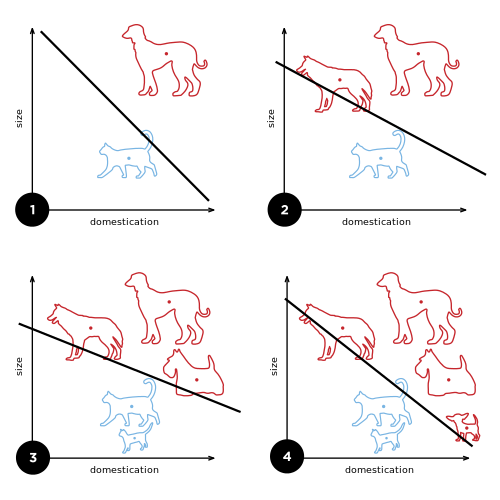
\includegraphics[width=0.9\textwidth]{images/Perceptron_example.svg.png}
       \end{figure}
          \end{column}
        \end{columns}
      \end{frame}

      \begin{frame}{Training von Neuronalen Netzen: Single-Layer-Perceptron}
        \begin{columns}
          \begin{column}{0.7\textwidth}
            \begin{itemize}
              \item Gegeben: Trainingsdatensatz $\mathcal{D} = \{(\mathbf{x}_i, y_i)\}_{i=1}^n$ mit $\mathbf{x}_i \in \mathbb{R}^d, y_i \in \{-1, +1\}$
              \item Perceptron-Lernregel \cite{rosenblatt1958}:
                    \begin{equation}
                       \mathbf{w}^{(t+1)} = \mathbf{w}^{(t)} + \eta \sum_{(\mathbf{x}_i, y_i) \in \mathcal{M}^{(t)}} y_i \mathbf{x}_i
                    \end{equation}
              \item Fehlklassifizierungen: $\mathcal{M}^{(t)} = \{(\mathbf{x}_i, y_i) : y_i(\mathbf{w}^{(t)T}\mathbf{x}_i + b) \leq 0\}$
              \item Verlustfunktion (Perceptron-Verlust):
              \begin{equation}
                L(\mathbf{w}, b) = \sum_{(\mathbf{x}_i, y_i) \in \mathcal{M}} -y_i(\mathbf{w}^T\mathbf{x}_i + b)
              \end{equation}
              \item Konvergenz-Theorem: Für linear separierbare Daten konvergiert der Algorithmus in endlich vielen Schritten
              \item Margin $\gamma = \min_{i} \frac{y_i(\mathbf{w}^*T\mathbf{x}_i + b^*)}{||\mathbf{w}^*||_2}$ bestimmt Konvergenzgeschwindigkeit
            \end{itemize}
          \end{column}
          \begin{column}{0.3\textwidth}
       \begin{figure}
       \centering
                   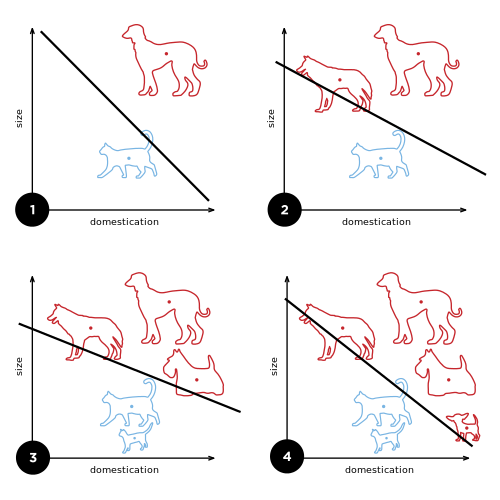
\includegraphics[width=0.9\textwidth]{images/Perceptron_example.svg.png}
       \end{figure}
          \end{column}
        \end{columns}
      \end{frame}

      \begin{frame}{Training von Neuronalen Netzen: Gradientenabstieg}
        \begin{columns}
          \begin{column}{0.7\textwidth}
            \begin{itemize}
              \item \textbf{Gradientenabstieg} (Gradient Descent) - allgemeines Optimierungsverfahren
              \item Iterative Aktualisierung der Parameter:
                    \begin{equation}
                       \boldsymbol{\theta}^{(t+1)} = \boldsymbol{\theta}^{(t)} - \eta \nabla_{\boldsymbol{\theta}} L(\boldsymbol{\theta}^{(t)})
                    \end{equation}
              \item $\eta > 0$: Lernrate (Schrittweite), $\boldsymbol{\theta}$: Parametervektor
              \item Gradient einer Funktion $f: \mathbb{R}^n \to \mathbb{R}$:
              \begin{equation}
                \nabla f(\mathbf{x}) = \left( \frac{\partial f}{\partial x_1}, \frac{\partial f}{\partial x_2}, \ldots, \frac{\partial f}{\partial x_n} \right)^T
              \end{equation}
              \item Gradient zeigt in Richtung des steilsten Anstiegs $\Rightarrow$ $-\nabla f$ zeigt zum lokalen Minimum
              \item Für Perceptron-Verlust: 
              \begin{align}
                \frac{\partial L}{\partial w_j} &= \sum_{(\mathbf{x}_i, y_i) \in \mathcal{M}} -y_i x_{ij} \\
                \nabla_{\mathbf{w}} L &= -\sum_{(\mathbf{x}_i, y_i) \in \mathcal{M}} y_i \mathbf{x}_i
              \end{align}
            \end{itemize}
          \end{column}
          \begin{column}{0.3\textwidth}
       \begin{figure}
       \centering
                   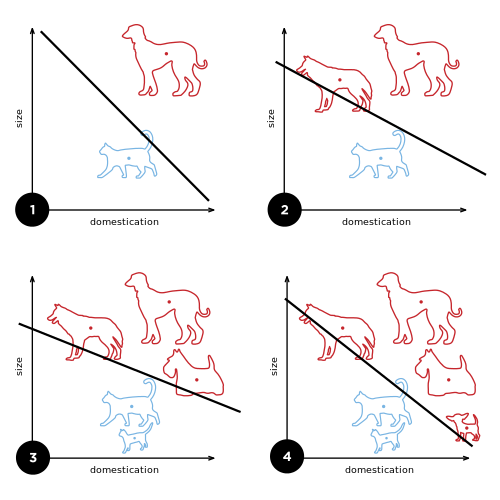
\includegraphics[width=0.9\textwidth]{images/Perceptron_example.svg.png}
       \end{figure}
          \end{column}
        \end{columns}
      \end{frame}

      \begin{frame}{Training von Neuronalen Netzen: Single-Layer-Perceptron}
        \begin{columns}
          \begin{column}{0.7\textwidth}
            \begin{itemize}

              \item Daraus folgt: \begin{align} 
                                  \nabla f(w) &= \left(  -\sum_{x \in F(w)} x_1,  -\sum_{x \in F(w)} x_2, ... ,  -\sum_{x \in F(w)} x_n   \right)
                                              &= -\sum_{x \in F(w)} x
                                  \end{align}
            \end{itemize}
          \end{column}
          \begin{column}{0.3\textwidth}
       \begin{figure}
       \centering
                   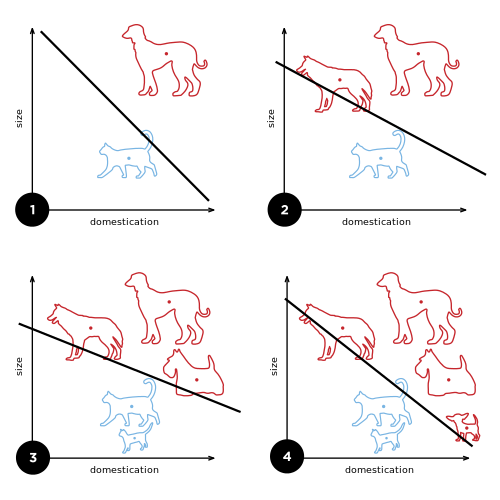
\includegraphics[width=0.9\textwidth]{images/Perceptron_example.svg.png}
       \end{figure}
          \end{column}
        \end{columns}
      \end{frame}

\begin{frame}{Grenzen des Single-Layer-Perceptrons -- Das XOR-Problem}
  \begin{columns}
    \begin{column}{0.6\textwidth}
      \begin{itemize}
        \item \textbf{Fundamentale Limitation}: Perceptron kann nur linear separierbare Probleme lösen
        \item \textbf{XOR-Problem} \cite{minsky1969}: 
        \begin{center}
        \begin{tabular}{|c|c|c|}
        \hline
        $x_1$ & $x_2$ & XOR \\
        \hline
        0 & 0 & 0 \\
        0 & 1 & 1 \\
        1 & 0 & 1 \\
        1 & 1 & 0 \\
        \hline
        \end{tabular}
        \end{center}
        \item \textbf{Mathematischer Beweis der Unmöglichkeit}: 
        \item Angenommen, es existiert $\mathbf{w} = (w_1, w_2)$ und $b$, sodass:
        \begin{align}
          w_1 \cdot 0 + w_2 \cdot 1 + b &> 0 \quad \text{(für (0,1))} \\
          w_1 \cdot 1 + w_2 \cdot 0 + b &> 0 \quad \text{(für (1,0))} \\
          w_1 \cdot 0 + w_2 \cdot 0 + b &\leq 0 \quad \text{(für (0,0))} \\
          w_1 \cdot 1 + w_2 \cdot 1 + b &\leq 0 \quad \text{(für (1,1))}
        \end{align}
        \item Aus (1) und (3): $w_2 > -b \geq 0 \Rightarrow w_2 > 0$
        \item Aus (2) und (3): $w_1 > -b \geq 0 \Rightarrow w_1 > 0$
        \item Aber (4): $w_1 + w_2 + b \leq 0$ \textbf{Widerspruch!}
      \end{itemize}
    \end{column}
    \begin{column}{0.4\textwidth}
      \begin{figure}
        \centering
                    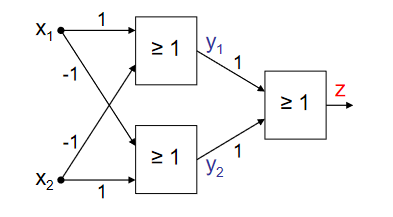
\includegraphics[width=0.9\textwidth]{images/XOR.png}
        \end{figure}
    \end{column}
  \end{columns}
\end{frame}

      \begin{frame}{Konstruktion von Neuronalen Netzen: Multi-Layer-Perceptron}
        \begin{columns}
          \begin{column}{0.7\textwidth}
            \begin{itemize}
              \item \textbf{Lösung des XOR-Problems}: Mehrschichtige Netze!
              \item \textbf{Komposition von Hyperebenen}: 
              \begin{itemize}
                \item Erste Schicht: Erzeugt mehrere lineare Entscheidungsgrenzen
                \item Zweite Schicht: Kombiniert diese zu komplexeren Formen
              \end{itemize}
              \item \textbf{Mathematische Intuition für XOR}:
              \begin{align}
                h_1 &= \sigma(x_1 + x_2 - 0.5) \quad \text{(OR-Gate)} \\
                h_2 &= \sigma(-x_1 - x_2 + 1.5) \quad \text{(NAND-Gate)} \\
                \text{XOR} &= \sigma(h_1 + h_2 - 1.5)
              \end{align}
              \item \textbf{Universal Approximation}: Mit einer versteckten Schicht können beliebige stetige Funktionen approximiert werden
              \item \textbf{Tiefe vs. Breite}: Tiefere Netze können effizienter sein als breitere
            \end{itemize}
          \end{column}
          \begin{column}{0.3\textwidth}
            \begin{figure}
              \centering
                          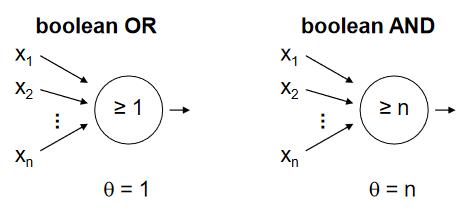
\includegraphics[width=0.9\textwidth]{images/OR_AND.png}
              \end{figure}
       \begin{figure}
       \centering
                   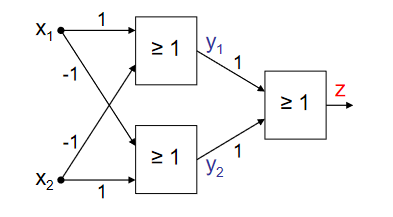
\includegraphics[width=0.9\textwidth]{images/XOR.png}
       \end{figure}
          \end{column}
        \end{columns}
      \end{frame}

      \begin{frame}{Training von Neuronalen Netzen: Multi-Layer-Perceptron}
        \begin{columns}
          \begin{column}{0.7\textwidth}
            \begin{itemize}
              \item \textbf{Multilayer Perceptron (MLP)}: Neuronales Netz mit versteckten Schichten
              \item Forward-Pass für 2-Schicht-Netz:
              \begin{align}
                \mathbf{z}^{(1)} &= \mathbf{W}^{(1)} \mathbf{x} + \mathbf{b}^{(1)} \quad \text{(lineare Transformation)} \\
                \mathbf{a}^{(1)} &= \sigma(\mathbf{z}^{(1)}) \quad \text{(Aktivierung)} \\
                \mathbf{z}^{(2)} &= \mathbf{W}^{(2)} \mathbf{a}^{(1)} + \mathbf{b}^{(2)} \\
                \hat{\mathbf{y}} &= \sigma(\mathbf{z}^{(2)})
              \end{align}
              \item Mean Squared Error (MSE) Loss:
              \begin{equation}
                L(\mathbf{W}, \mathbf{b}) = \frac{1}{n} \sum_{i=1}^{n} ||\hat{\mathbf{y}}_i - \mathbf{y}_i||_2^2
              \end{equation}
              \item Problem der Heaviside-Funktion: $H(x) = \begin{cases}1 & x \geq 0\\0 & x < 0\end{cases}$ nicht differenzierbar
              \item Lösung: Glatte Aktivierungsfunktionen (Sigmoid, Tanh, ReLU)
            \end{itemize}
          \end{column}
          \begin{column}{0.3\textwidth}
            \begin{figure}
              \centering
                          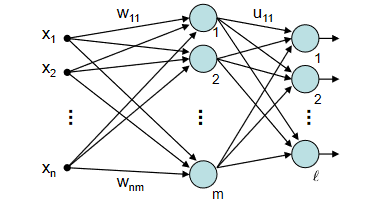
\includegraphics[width=0.9\textwidth]{images/MLP.png}
              \end{figure}
          \end{column}
        \end{columns}
      \end{frame}

      \begin{frame}{Training von Neuronalen Netzen: Multi-Layer-Perceptron}
        \begin{columns}
          \begin{column}{0.7\textwidth}
            \begin{itemize}
              \item
              \begin{equation}
                f(w) = \sum_{x\in B} || g(w; x) - g^*(x) ||^2 \quad \rightarrow \text{  min  }
              \end{equation} 
              \item mit dem Output des Netzes $ g(w;x) $ und dem erwarteten Output $ g^*(x) $ 
              \item 
              \begin{align}
                 u^{(t+1)} &= u^t - \gamma \nabla_u f(w_t , u_t) \\
                 w^{(t+1)} &= w^t - \gamma \nabla_w f(w_t , u_t) \\
              \end{align}
              \item $x_i$: Inputs 
              \item $y_j$: Werte nach dem ersten Layer
              \item $z_k$: Werte nach dem zweiten Layer
            \end{itemize}
          \end{column}
          \begin{column}{0.3\textwidth}
            \begin{figure}
              \centering
                          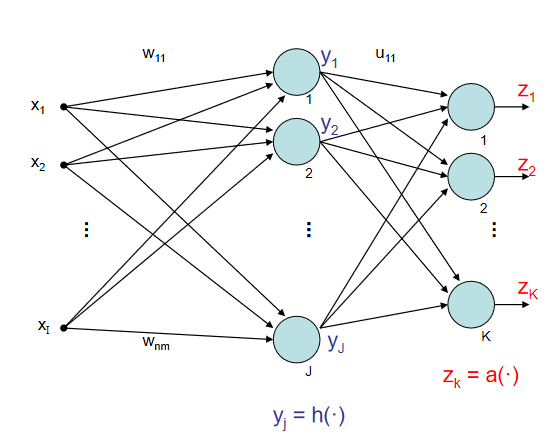
\includegraphics[width=0.9\textwidth]{images/MLP2.png}
              \end{figure}
          \end{column}
        \end{columns}
      \end{frame}

      \begin{frame}{Backpropagation-Algorithmus: Mathematische Grundlagen}
        \begin{columns}
          \begin{column}{1\textwidth}
            \begin{itemize}
              \item \textbf{Backpropagation} \cite{rumelhart1986}: Effizienter Algorithmus zur Berechnung von Gradienten in neuronalen Netzen
              \item Anwendung der Kettenregel der Differentiation:
              \begin{equation}
                \frac{\partial L}{\partial w_{ij}^{(l)}} = \frac{\partial L}{\partial z_j^{(l)}} \cdot \frac{\partial z_j^{(l)}}{\partial w_{ij}^{(l)}}
              \end{equation}
              \item Definition der \textbf{lokalen Gradienten} (Deltas):
              \begin{equation}
                \delta_j^{(l)} = \frac{\partial L}{\partial z_j^{(l)}}
              \end{equation}
              \item Rekursive Berechnung (rückwärts durch das Netz):
              \begin{align}
                \delta_j^{(L)} &= \frac{\partial L}{\partial a_j^{(L)}} \cdot \sigma'(z_j^{(L)}) \quad \text{(Output-Schicht)} \\
                \delta_j^{(l)} &= \left(\sum_{k} \delta_k^{(l+1)} w_{jk}^{(l+1)}\right) \sigma'(z_j^{(l)}) \quad \text{(versteckte Schichten)}
              \end{align}
              \item Gradientenberechnung:
              \begin{align}
                \frac{\partial L}{\partial w_{ij}^{(l)}} &= \delta_j^{(l)} \cdot a_i^{(l-1)} \\
                \frac{\partial L}{\partial b_j^{(l)}} &= \delta_j^{(l)}
              \end{align}
            \end{itemize}
          \end{column}
          %\begin{column}{0.3\textwidth}
          %  \begin{figure}
          %    \centering
          %                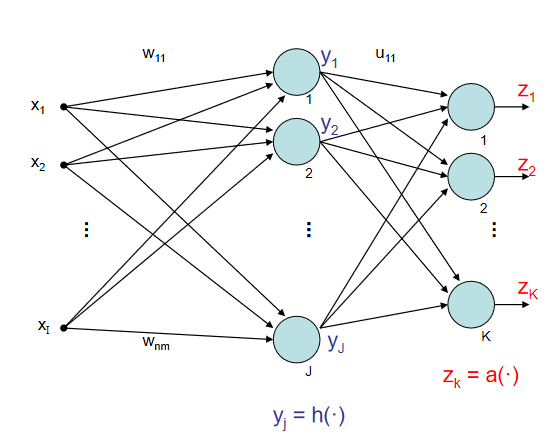
\includegraphics[width=0.9\textwidth]{images/MLP2.png}
          %    \end{figure}
          %\end{column}
        \end{columns}
      \end{frame}

      \begin{frame}{Training von Neuronalen Netzen: Multi-Layer-Perceptron}
        \begin{columns}
          \begin{column}{1\textwidth}
            \begin{itemize}
              \item analog zum SLP nutzen wir den Gradienten zur Minimierung des Fehlers
            \begin{align*}
              \nabla f(w,u) &= \sum_{x,z^* \in B} \nabla f(w, u; x,z^*) \\
              \frac{\partial f(w,u)}{\partial u_{jk}} &= \sum_{x,z^* \in B} \frac{\partial f(w,u;x,z^*)}{\partial u_{jk}} \\
              \frac{\partial f(w,u)}{\partial w_{ij}} &= \sum_{x,z^* \in B} \frac{\partial f(w,u;x,z^*)}{\partial w_{ij}} 
            \end{align*}
            \item mit den Sigmoid-Aktivierungsfunktionen:
            \begin{align*}
              a(x) = h(x) = \frac{1}{1+e^{-x}} \text{mit der Ableitung:  } \frac{\text{d}a(x)}{\text{dx}} = a(x) \cdot (1 - a(x))
            \end{align*}
            \item mit der Kettenregel für Ableitungen:
            \begin{equation*}
              [p(q(x))]´ = p´(q(x)) \cdot q´(x) 
            \end{equation*}
            \item ergibt sich für den Gradienten von $f$:
            \begin{align*}
              f(w,u;x,z^*) &= \sum_{k=1} ^K [a(u_k y) - z^*_k]^2 \\
              \frac{\partial f(w,u; x,z^*) }{ \partial u_{jk} } &= \sum_{x,z^* \in B} \frac{\partial f(w,u;x,z^*)}{\partial u_{jk}} \\
                                                            &= 2 [a(u´_k y)-z^*_k] \cdot a´(u´_k y) \cdot y_j \\
                                                            &= 2 [a(u´_k y)-z^*_k] \cdot a(u´_k y \cdot (1 - a(u´_k y)))\cdot y_j\\
                                                            &=  \underbrace{ 2 [z_k - z^*_k] \cdot z_k \cdot (1- z_k) }_\text{Fehlerterm $ \delta_k$} \cdot y_j \\
               \frac{\partial f(w,u; x,z^*)}{\partial w_{ij}} &= 2 \sum_{k=1} ^K (a(u´_k y) -z^*_k) \cdot a´(u´_k y) \cdot u_{jk} \cdot h´(w´_j x) x_i \\
                                                             &= 2 \sum_{k=1} ^K ( z_k -z^*_k) \cdot z_k \cdot (1-z_k) \cdot u_{jk} \cdot y_j (1-y_j) x_i \\                                                            
                                                             &= x_i y_j (1-y_j)  \underbrace{2 \sum_{k=1} ^K ( z_k -z^*_k) \cdot z_k \cdot (1-z_k) }_\text{Fehlerterm $ \delta_i$} \cdot u_{jk} \cdot y_j 
            \end{align*}
            \end{itemize}
          \end{column}
          %\begin{column}{0.3\textwidth}
          %  \begin{figure}
          %    \centering
          %                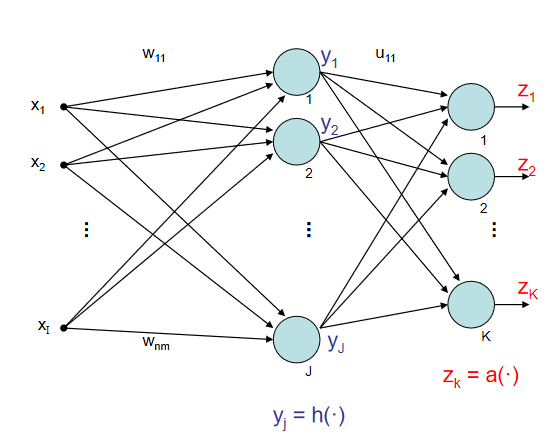
\includegraphics[width=0.9\textwidth]{images/MLP2.png}
          %    \end{figure}
          %\end{column}
        \end{columns}
      \end{frame}
      \begin{frame}{Training von Neuronalen Netzen: Multi-Layer-Perceptron}
        \begin{columns}
          \begin{column}{1\textwidth}
            \begin{itemize}

            \item ergibt sich für den Gradienten von $f$:
            \begin{align*}
              f(w,u;x,z^*) &= \sum_{k=1} ^K [a(u_k y) - z^*_k]^2 \\
              \frac{\partial f(w,u; x,z^*) }{ \partial u_{jk} } &= \sum_{x,z^* \in B} \frac{\partial f(w,u;x,z^*)}{\partial u_{jk}} \\
                                                            &= 2 [a(u´_k y)-z^*_k] \cdot a´(u´_k y) \cdot y_j \\
                                                            &= 2 [a(u´_k y)-z^*_k] \cdot a(u´_k y \cdot (1 - a(u´_k y)))\cdot y_j\\
                                                            &=  \underbrace{ 2 [z_k - z^*_k] \cdot z_k \cdot (1- z_k) }_\text{Fehlerterm $ \delta_k$} \cdot y_j \\
               \frac{\partial f(w,u; x,z^*)}{\partial w_{ij}} &= 2 \sum_{k=1} ^K (a(u´_k y) -z^*_k) \cdot a´(u´_k y) \cdot u_{jk} \cdot h´(w´_j x) x_i \\
                                                             &= 2 \sum_{k=1} ^K ( z_k -z^*_k) \cdot z_k \cdot (1-z_k) \cdot u_{jk} \cdot y_j (1-y_j) x_i \\                                                            
                                                             &= x_i y_j (1-y_j)  \underbrace{2 \sum_{k=1} ^K ( z_k -z^*_k) \cdot z_k \cdot (1-z_k) }_\text{Fehlerterm $ \delta_i$} \cdot u_{jk} \cdot y_j 
            \end{align*}
            \end{itemize}
          \end{column}
          %\begin{column}{0.3\textwidth}
          %  \begin{figure}
          %    \centering
          %                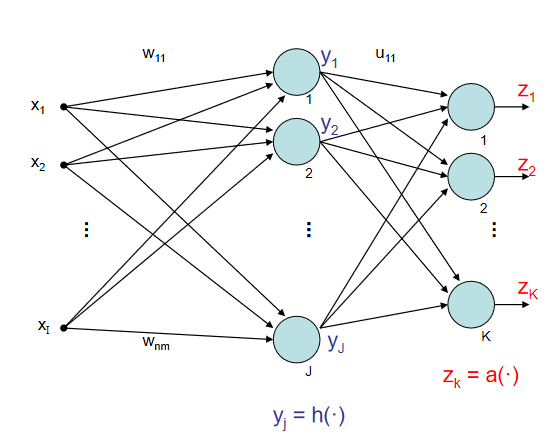
\includegraphics[width=0.9\textwidth]{images/MLP2.png}
          %    \end{figure}
          %\end{column}
        \end{columns}
      \end{frame}

      \begin{frame}{ Verallgemeinerung Training von Neuronalen Netzen: M-Layer-Perceptron}
        \begin{columns}
          \begin{column}{1\textwidth}
            \begin{itemize}
              \item bei einem Neuronalen Netz mi $L$ Layern $S_1, S_2 , ... , S_L$
              \item den Gewichten $w_{ij}$ in der Matrix $W$
              \item dem output eines Neurons $o_j$
              \item ist der Fehlerterm: 
            \begin{equation*}
              \delta_j = \begin{cases} o_j \cdot (1-o_j) \cdot  (o_j -z_j*) & \text{if }\ j \in S_L, \text{output Neuron} \\ o_j \cdot (1-o_j) \cdot \sum_{k \in S_{m+1}} \delta_k \cdot w_{jk} & \text{if } j \in S_m \text{and } m<L \end{cases}
            \end{equation*}
            \item Der Korrekturterm für die einzelnen Gewichte ist dann:
            \begin{equation}
              w_{ij}^{(t+1)} = w_{ij}^{t} - \gamma \cdot o_i \cdot \delta_j 
            \end{equation}
            \end{itemize}
          \end{column}
          %\begin{column}{0.3\textwidth}
          %  \begin{figure}
          %    \centering
          %                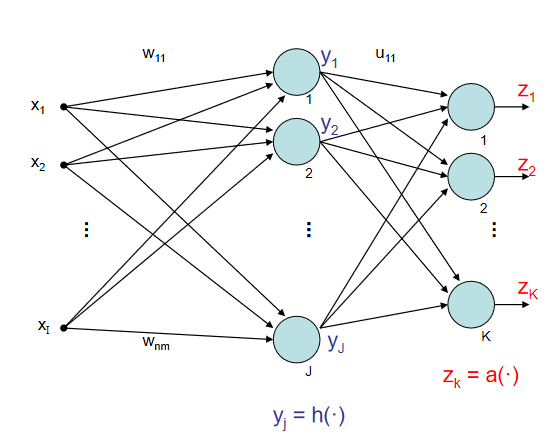
\includegraphics[width=0.9\textwidth]{images/MLP2.png}
          %    \end{figure}
          %\end{column}
        \end{columns}
      \end{frame}

      \begin{frame}{Fortgeschrittene Optimierungsalgorithmen}
        \begin{columns}
          \begin{column}{1\textwidth}
            \begin{itemize}
              \item \textbf{Momentum}: Beschleunigung in konsistente Richtungen
              \begin{align}
                \mathbf{v}^{(t+1)} &= \beta \mathbf{v}^{(t)} + \eta \nabla L(\boldsymbol{\theta}^{(t)}) \\
                \boldsymbol{\theta}^{(t+1)} &= \boldsymbol{\theta}^{(t)} - \mathbf{v}^{(t+1)}
              \end{align}
              \item \textbf{ADAM} \cite{kingma2014adam} (Adaptive Moment Estimation) - Kombination aus Momentum und RMSprop:
              \begin{align}
                m_w^{(t+1)} &= \beta_1 m_w^{(t)} + (1 - \beta_1) \nabla_w L^{(t)} \quad \text{(1. Moment)} \\
                v_w^{(t+1)} &= \beta_2 v_w^{(t)} + (1 - \beta_2) (\nabla_w L^{(t)})^2 \quad \text{(2. Moment)} \\
                \hat{m}_w^{(t)} &= \frac{m_w^{(t+1)}}{1 - \beta_1^{t+1}} \quad \text{(Bias-Korrektur)} \\
                \hat{v}_w^{(t)} &= \frac{v_w^{(t+1)}}{1 - \beta_2^{t+1}} \quad \text{(Bias-Korrektur)} \\
                w^{(t+1)} &= w^{(t)} - \frac{\eta}{\sqrt{\hat{v}_w^{(t)}} + \epsilon} \hat{m}_w^{(t)}
              \end{align}
              \item Typische Hyperparameter: $\beta_1 = 0.9$, $\beta_2 = 0.999$, $\epsilon = 10^{-8}$
            \end{itemize}
          \end{column}
          % \begin{column}{0.3\textwidth}
          %   \begin{figure}
          %     \centering
          %                 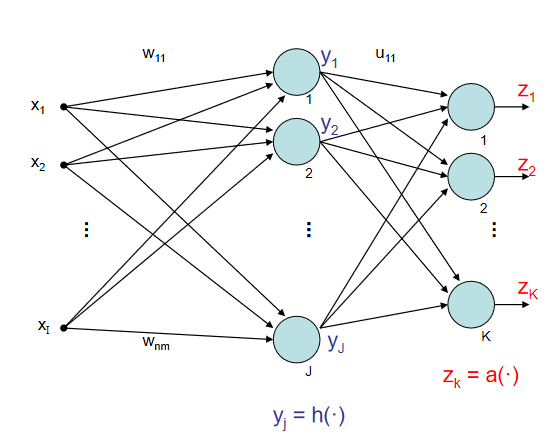
\includegraphics[width=0.9\textwidth]{images/MLP2.png}
          %     \end{figure}
          % \end{column}
        \end{columns}
      \end{frame}

\begin{frame}{Warum "Deep" Learning? -- Mathematische Rechtfertigung für tiefe Netze}
  \begin{columns}
    \begin{column}{1\textwidth}
      \begin{itemize}
        \item \textbf{Representation Learning}: Tiefere Netze lernen hierarchische Merkmalsdarstellungen
        \item \textbf{Mathematischer Vorteil}: Exponentiell weniger Parameter für dieselbe Expressivität
        \item \textbf{Beispiel - Parität-Funktion}: Prüfe, ob eine ungerade Anzahl von Bits gesetzt ist
        \begin{itemize}
          \item Flaches Netz: Benötigt $O(2^n)$ versteckte Neuronen
          \item Tiefes Netz: Benötigt nur $O(n)$ Neuronen in $O(\log n)$ Schichten
        \end{itemize}
        \item \textbf{Kompositionelle Struktur}: Viele reale Funktionen haben hierarchische Struktur
        \begin{equation}
          f(\mathbf{x}) = g_L(g_{L-1}(...g_2(g_1(\mathbf{x}))...))
        \end{equation}
        \item \textbf{Feature Learning}: Jede Schicht $\ell$ lernt Features der Form:
        \begin{equation}
          \mathbf{h}^{(\ell)} = \sigma(\mathbf{W}^{(\ell)} \mathbf{h}^{(\ell-1)} + \mathbf{b}^{(\ell)})
        \end{equation}
        \item \textbf{Intuition}: 
        \begin{itemize}
          \item Untere Schichten: Einfache Features (Kanten, Texturen)
          \item Mittlere Schichten: Kombinationen (Formen, Teile)
          \item Obere Schichten: Komplexe Konzepte (Objekte, Semantik)
        \end{itemize}
      \end{itemize}
    \end{column}
  \end{columns}
\end{frame}

      \begin{frame}{Das Vanishing Gradient Problem -- Warum tiefe Netze schwer zu trainieren sind}
        \begin{columns}
          \begin{column}{0.6\textwidth}
            \begin{itemize}
              \item \textbf{Problem}: Bei tiefen Netzen werden Gradienten exponentiell kleiner
              \item \textbf{Mathematische Analyse}: Für Sigmoid-Aktivierung $\sigma'(x) \leq 0.25$
              \item Gradient in Schicht $\ell$ proportional zu:
              \begin{equation}
                \frac{\partial L}{\partial \mathbf{W}^{(\ell)}} \propto \prod_{i=\ell+1}^{L} \mathbf{W}^{(i)} \sigma'(\mathbf{z}^{(i)})
              \end{equation}
              \item Für $L-\ell$ Schichten: Faktor $\leq (0.25)^{L-\ell}$ 
              \item \textbf{Beispiel}: Bei 10 Schichten kann Gradient um Faktor $10^{-6}$ schrumpfen!
              \item \textbf{Lösungsansätze}:
              \begin{itemize}
                \item ReLU-Aktivierungen: $\text{ReLU}'(x) = 1$ für $x > 0$
                \item Residual Connections (ResNets)
                \item Normalization (BatchNorm, LayerNorm)
                \item Bessere Initialisierung (Xavier, He)
              \end{itemize}
            \end{itemize}
          \end{column}
           \begin{column}{0.4\textwidth}
             \begin{figure}
               \centering
                           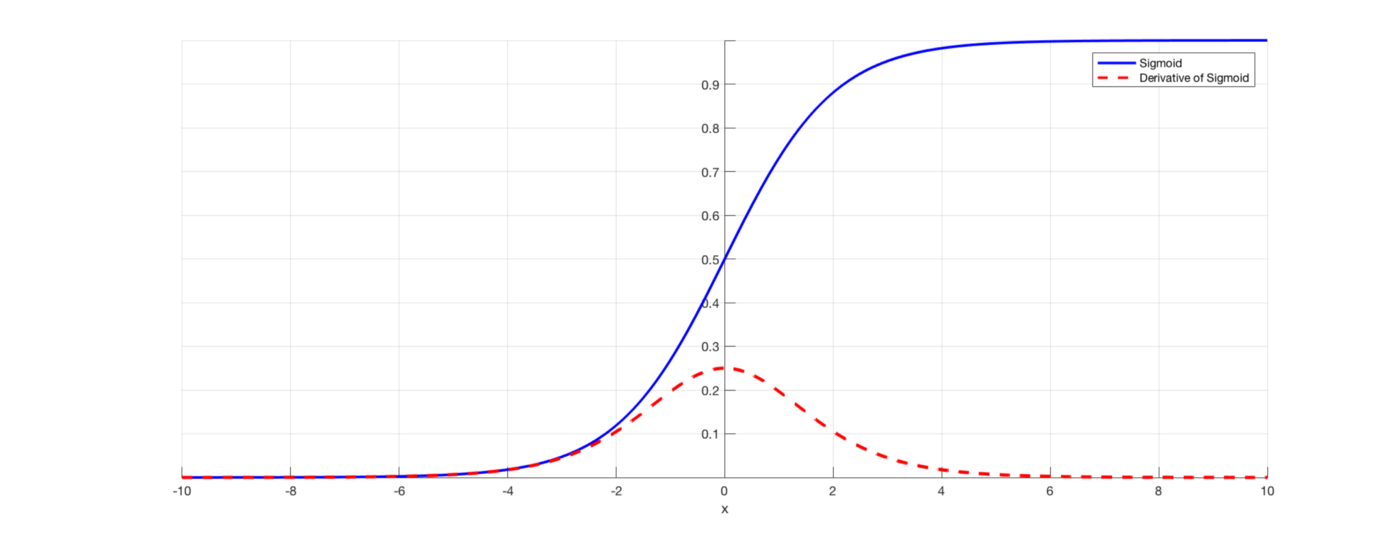
\includegraphics[width=0.9\textwidth]{images/sigmoid.png}
               \end{figure}
           \end{column}
        \end{columns}
      \end{frame}

      \begin{frame}{Aktivierungsfunktionen -- Mathematische Eigenschaften und Warum sie wichtig sind}
        \begin{columns}
          \begin{column}{1\textwidth}
            \begin{itemize}
              \item \textbf{Sigmoid-Funktion}: $\sigma(x) = \frac{1}{1 + e^{-x}}$, Ableitung: $\sigma'(x) = \sigma(x)(1-\sigma(x))$
              \begin{itemize}
                \item Glatt und differenzierbar, Ausgabe in $(0,1)$
                \item \textbf{Problem}: Vanishing Gradients für $|x| >> 0$: $\sigma'(x) \to 0$
              \end{itemize}
              \item \textbf{Tanh-Funktion}: $\tanh(x) = \frac{e^x - e^{-x}}{e^x + e^{-x}}$, Ableitung: $\tanh'(x) = 1 - \tanh^2(x)$
              \begin{itemize}
                \item Ausgabe in $(-1,1)$, zero-centered (bessere Konvergenz)
                \item Ebenfalls Vanishing Gradient Problem
              \end{itemize}
              \item \textbf{ReLU-Funktion} \cite{nair2010}: $\text{ReLU}(x) = \max(0,x)$, Ableitung: $\text{ReLU}'(x) = \begin{cases} 1 & x > 0 \\ 0 & x \leq 0 \end{cases}$
              \begin{itemize}
                \item Löst Vanishing Gradient Problem für $x > 0$
                \item Computationally efficient, führt zu sparse representations
                \item \textbf{Problem}: "Dying ReLU" - Neuronen können "sterben" wenn $x \leq 0$
              \end{itemize}
              \item \textbf{Warum Nichtlinearität essentiell ist}:
              \begin{equation}
                \text{Ohne } \sigma: f(\mathbf{x}) = \mathbf{W}_2(\mathbf{W}_1 \mathbf{x}) = (\mathbf{W}_2\mathbf{W}_1)\mathbf{x} = \mathbf{W}_{\text{linear}}\mathbf{x}
              \end{equation}
            \end{itemize}
          \end{column}
        \end{columns}
      \end{frame}

      \begin{frame}{Häufige Aktivierungsfunktionen -- Visualisierung}
        \begin{columns}
          \begin{column}{0.5\textwidth}
            \begin{figure}
              \centering
                          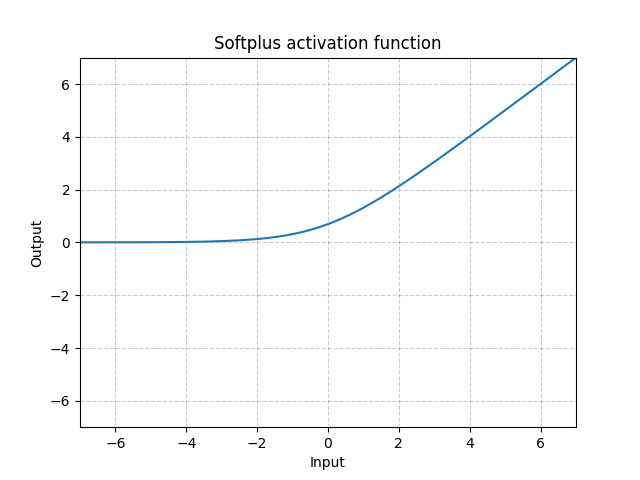
\includegraphics[width=0.9\textwidth]{images/Softplus.png}
              \end{figure}
          \end{column}
           \begin{column}{0.5\textwidth}
             \begin{figure}
               \centering
                           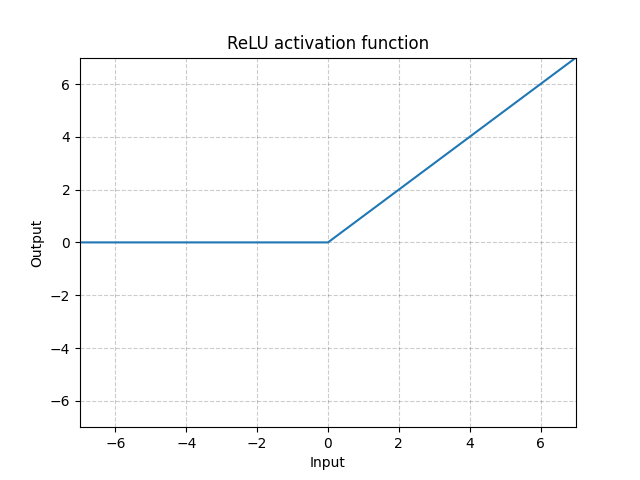
\includegraphics[width=0.9\textwidth]{images/ReLU.png}
               \end{figure}
           \end{column}
        \end{columns}
      \end{frame}

      
      \begin{frame}{Weitere Netzwerk Architekturen}
        \begin{columns}
          \begin{column}{0.6\textwidth}
            \begin{itemize}
              \item spezielle Datenstrukturen profitieren von speziellen Architekturen \newline 
              \item Bilderkennung \rightarrow Convolutional Neural Network (CNN) \newline 
              \item sequentielle Daten \rightarrow Recurrent Neural Networks (RNN) \newline 
              \item im speziellen um Kausalität/Kontext herzustellen \rightarrow Long Short Term Memory (LSTM) \newline
            \end{itemize}
          \end{column}
           \begin{column}{0.4\textwidth}
             \begin{figure}
               \centering
                           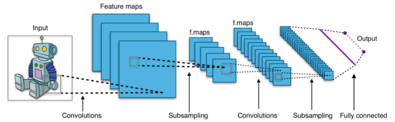
\includegraphics[width=0.9\textwidth]{images/CNN.png}
               \end{figure}
               \begin{figure}
                \centering
                            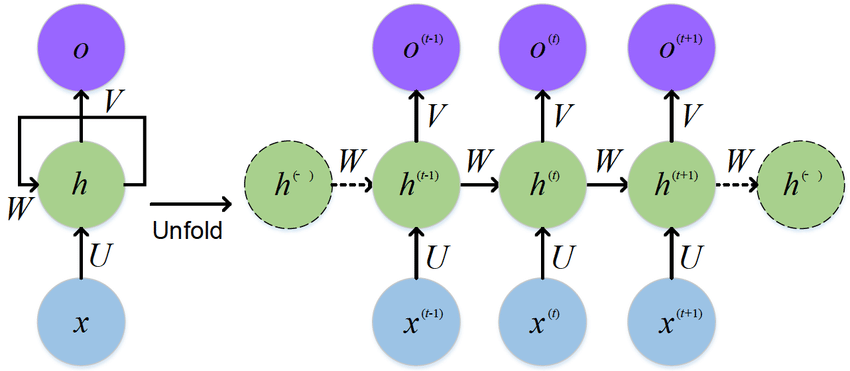
\includegraphics[width=0.9\textwidth]{images/RNN.png}
                \end{figure}
           \end{column}
        \end{columns}
      \end{frame}

      \begin{frame}{Warum funktionieren CNNs? -- Mathematische Prinzipien}
        \begin{columns}
          \begin{column}{1\textwidth}
            \begin{itemize}
              \item \textbf{Drei Schlüsselprinzipien von CNNs}:
              \item \textbf{1. Lokale Konnektivität}: Jedes Neuron ist nur mit lokalem Bereich verbunden
              \begin{equation}
                y_{i,j}^{(\ell)} = \sigma\left(\sum_{m=-k}^{k} \sum_{n=-k}^{k} w_{m,n}^{(\ell)} \cdot x_{i+m,j+n}^{(\ell-1)} + b^{(\ell)}\right)
              \end{equation}
              \item \textbf{2. Parameter Sharing}: Derselbe Filter $\mathbf{W}$ wird über gesamte Feature-Map verwendet
              \begin{itemize}
                \item Reduziert Parameter von $O(H \cdot W \cdot d^2)$ auf $O(k^2 \cdot d)$
                \item Erzwingt Translationsinvarianz
              \end{itemize}
              \item \textbf{3. Equivarianz zu Translationen}: Wenn Input um $\mathbf{t}$ verschoben wird, verschiebt sich Output ebenfalls um $\mathbf{t}$
              \begin{equation}
                \text{Conv}(T_\mathbf{t}[\mathbf{x}]) = T_\mathbf{t}[\text{Conv}(\mathbf{x})]
              \end{equation}
              \item \textbf{Pooling} führt zu begrenzter Translationsinvarianz:
              \begin{equation}
                \text{MaxPool}(\mathbf{X})_{i,j} = \max_{(p,q) \in \mathcal{N}_{i,j}} \mathbf{X}_{p,q}
              \end{equation}
              \item \textbf{Hierarchische Feature-Extraktion}: Einfache → Komplexe Features
            \end{itemize}
          \end{column}
        \end{columns}
      \end{frame}

      \begin{frame}{Spezielle Netzwerkarchitekturen: CNN -- Implementierung}
        \begin{columns}
          \begin{column}{0.6\textwidth}
            \begin{itemize}
              \item \textbf{Convolutional Neural Networks} \cite{lecun1998}: Spezialisiert auf gitterförmige Daten (Bilder) \newline
              \item \textbf{Faltungsoperation} (2D-Convolution):
              \begin{equation}
                (\mathbf{I} * \mathbf{K})_{i,j} = \sum_{m=0}^{M-1} \sum_{n=0}^{N-1} \mathbf{I}_{i+m,j+n} \cdot \mathbf{K}_{m,n}
              \end{equation}
              \item $\mathbf{I}$: Input-Feature-Map, $\mathbf{K}$: Kernel (Filter) der Größe $M \times N$ \newline
              \item \textbf{Pooling}: Dimensionsreduktion, z.B. Max-Pooling:
              \begin{equation}
                \text{MaxPool}(\mathbf{X})_{i,j} = \max_{p,q \in P_{i,j}} \mathbf{X}_{p,q}
              \end{equation}
              \item \textbf{Parameter Sharing}: Derselbe Filter wird über gesamte Feature-Map angewendet
              \item \textbf{Translation Invariance}: Robustheit gegenüber Verschiebungen
            \end{itemize}
          \end{column}
           \begin{column}{0.4\textwidth}
             \begin{figure}
               \centering
                           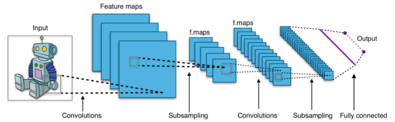
\includegraphics[width=0.9\textwidth]{images/CNN.png}
               \end{figure}
               \begin{figure}
                \centering
                            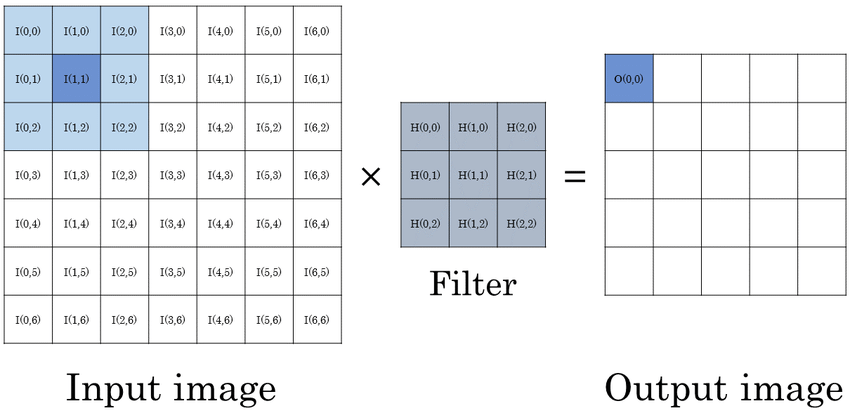
\includegraphics[width=0.9\textwidth]{images/convolution.png}
                \end{figure}
           \end{column}
        \end{columns}
      \end{frame}

      \begin{frame}{Spezielle Netzwerkarchitekturen: CNN}
        \begin{columns}
          \begin{column}{0.5\textwidth}
            \begin{itemize}
              \item Anschaulich: Formen werden erkannt \newline 
              \item Katzenohren sind anders als Hundeohren \newline 
              \item Verallgemeinerbar für andere Objektklassifizierungen \newline
            \end{itemize}
          \end{column}
           \begin{column}{0.5\textwidth}
             \begin{figure}
               \centering
                           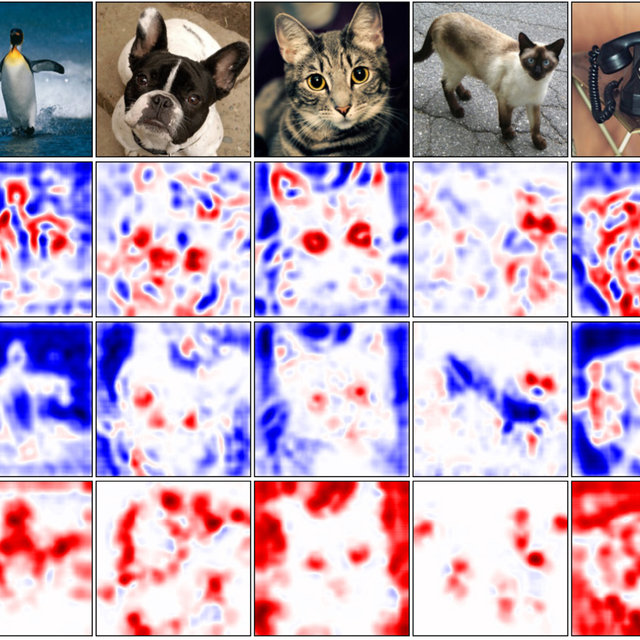
\includegraphics[width=0.9\textwidth]{images/featuremaps.jpg}
               \end{figure}

           \end{column}
        \end{columns}
      \end{frame}

      \begin{frame}{Spezielle Netzwerkarchitekturen: RNN}
        \begin{columns}
          \begin{column}{0.6\textwidth}
            \begin{itemize}
              \item Anschaulich: Schleife in Netzwerk "merkt" sich voherige Zustände \newline 
              \item funktioniert für kurze Zeiträume \newline 
              \item Entfaltung eines RNN \rightarrow viele zu trainierende Gewichte \newline 
              \item Problem: langfristige Zusammenhänge werden nicht erfasst \newline 
              \item Problem: Verschwindende Gradienten
            \end{itemize}
          \end{column}
           \begin{column}{0.4\textwidth}
             \begin{figure}
               \centering
                           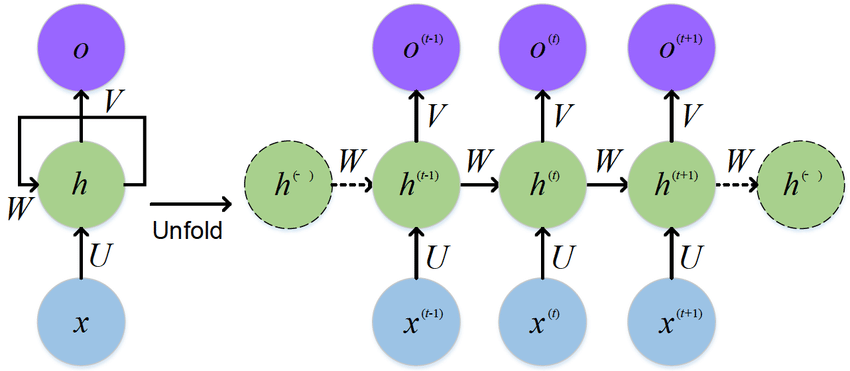
\includegraphics[width=0.9\textwidth]{images/RNN.png}
               \end{figure}

           \end{column}
        \end{columns}
      \end{frame}     
      
      \begin{frame}{Spezielle Netzwerkarchitekturen: LSTM}
        \begin{columns}
          \begin{column}{0.6\textwidth}
            \begin{itemize}
              \item \textbf{Long Short-Term Memory} \cite{hochreiter1997}: Lösung des Vanishing Gradient Problems in RNNs \newline
              \item \textbf{Cell State} $\mathbf{C}_t$: Langzeit-Gedächtnis der LSTM-Zelle \newline
              \item \textbf{Hidden State} $\mathbf{h}_t$: Kurzzeit-Output der Zelle \newline
              \item Drei Gating-Mechanismen kontrollieren Informationsfluss:
              \begin{itemize}
                \item Forget Gate: Welche Informationen vergessen?
                \item Input Gate: Welche neuen Informationen speichern?
                \item Output Gate: Welche Teile des Cell States ausgeben?
              \end{itemize}
            \end{itemize}
          \end{column}
           \begin{column}{0.4\textwidth}
             \begin{figure}
               \centering
                           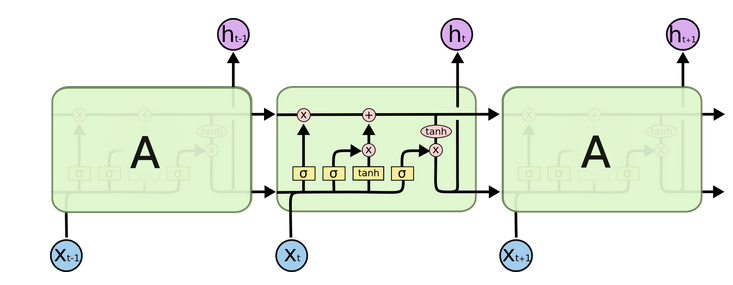
\includegraphics[width=0.9\textwidth]{images/LSTM_1.png}
               \end{figure}
               \begin{figure}
                \centering
                            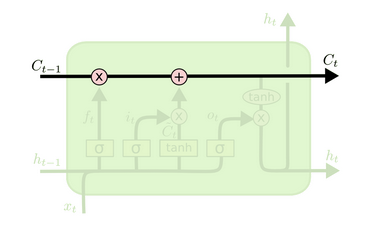
\includegraphics[width=0.9\textwidth]{images/LSTM_2.png}
                \end{figure}

           \end{column}
        \end{columns}
      \end{frame}
      
            
      \begin{frame}{LSTM: Mathematische Formulierung}
        \begin{columns}
          \begin{column}{0.6\textwidth}
            \begin{itemize}              
              \item \textbf{Forget Gate}: Entscheidet, welche Informationen aus $\mathbf{C}_{t-1}$ gelöscht werden
              \begin{equation}
                \mathbf{f}_t = \sigma(\mathbf{W}_f \cdot [\mathbf{h}_{t-1}, \mathbf{x}_t] + \mathbf{b}_f)
              \end{equation}
              \item \textbf{Input Gate}: Bestimmt neue Informationen für Cell State
              \begin{align}
                \mathbf{i}_t &= \sigma(\mathbf{W}_i \cdot [\mathbf{h}_{t-1}, \mathbf{x}_t] + \mathbf{b}_i) \\
                \tilde{\mathbf{C}}_t &= \tanh(\mathbf{W}_C \cdot [\mathbf{h}_{t-1}, \mathbf{x}_t] + \mathbf{b}_C)
              \end{align}
              \item \textbf{Cell State Update}:
              \begin{equation}
                \mathbf{C}_t = \mathbf{f}_t * \mathbf{C}_{t-1} + \mathbf{i}_t * \tilde{\mathbf{C}}_t
              \end{equation}
              \item \textbf{Output Gate} und \textbf{Hidden State}:
              \begin{align}
                \mathbf{o}_t &= \sigma(\mathbf{W}_o \cdot [\mathbf{h}_{t-1}, \mathbf{x}_t] + \mathbf{b}_o) \\
                \mathbf{h}_t &= \mathbf{o}_t * \tanh(\mathbf{C}_t)
              \end{align}
            \end{itemize}
          \end{column}
           \begin{column}{0.4\textwidth}
             \begin{figure}
               \centering
                           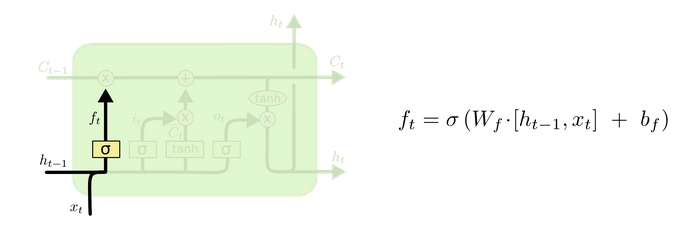
\includegraphics[width=0.9\textwidth]{images/LSTM_3.png}
               \end{figure}
               \begin{figure}
                \centering
                            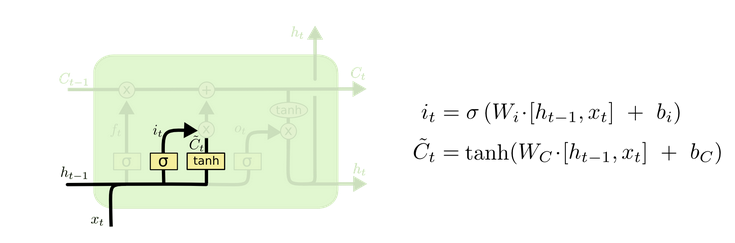
\includegraphics[width=0.9\textwidth]{images/LSTM_4.png}
                \end{figure}
            

           \end{column}
        \end{columns}
      \end{frame} 

      \begin{frame}{Spezielle Netzwerkarchitekturen: LSTM}
        \begin{columns}
          \begin{column}{0.6\textwidth}
            \begin{itemize}
             
              \item Update des alten Cell states mithilfe des alten und neuen Zustandes \newline 
              \item Output der LSTM Zelle und Erzeugung des neuen hidden states \newline 
            \end{itemize}
          \end{column}
           \begin{column}{0.4\textwidth}
            
               \begin{figure}
                \centering
                            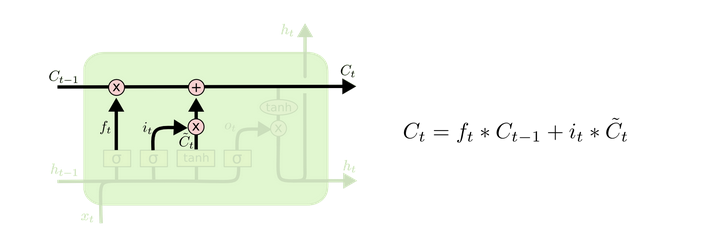
\includegraphics[width=0.9\textwidth]{images/LSTM_5.png}
                \end{figure}
                \begin{figure}
                  \centering
                              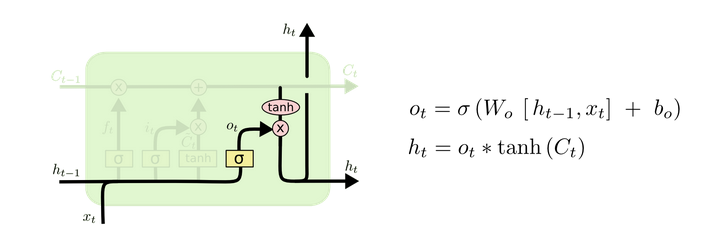
\includegraphics[width=0.9\textwidth]{images/LSTM_6.png}
                  \end{figure}

           \end{column}
        \end{columns}
      \end{frame} 


      \begin{frame}{Spezielle Netzwerkarchitekturen: Unsupervised Learning}
        \begin{columns}
          \begin{column}{0.6\textwidth}
            \begin{itemize}
              \item Autoencoder bzw. Encoder-Decoder Netzwerke \newline
              \item Versuch den Input wieder zu rekonstruieren \rightarrow Interessant für unsupervised anomaly detection \newline 
              \item Generative Netzwerk \newline
              \item Möglichkeit aus "Noise" komplexe echt aussehende Daten zu erzeugen \rightarrow mögliche Beschleunigung von (FE-)Simulationen
            \end{itemize}
          \end{column}
           \begin{column}{0.4\textwidth}
             \begin{figure}
               \centering
                           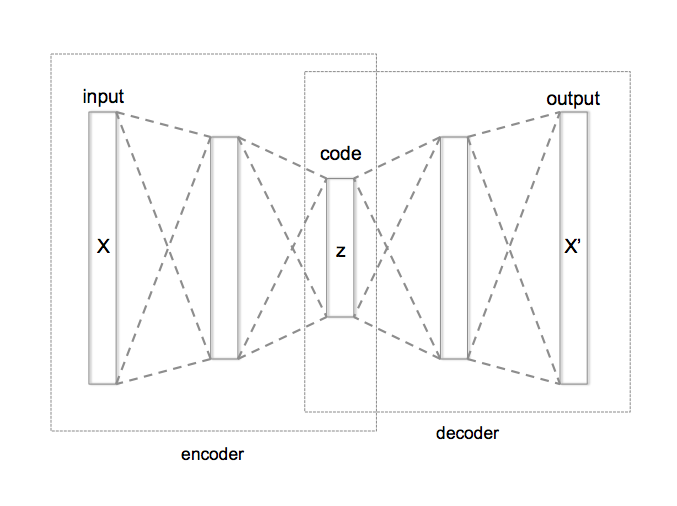
\includegraphics[width=0.9\textwidth]{images/Autoencoder.png}
               \end{figure}
               \begin{figure}
                \centering
                            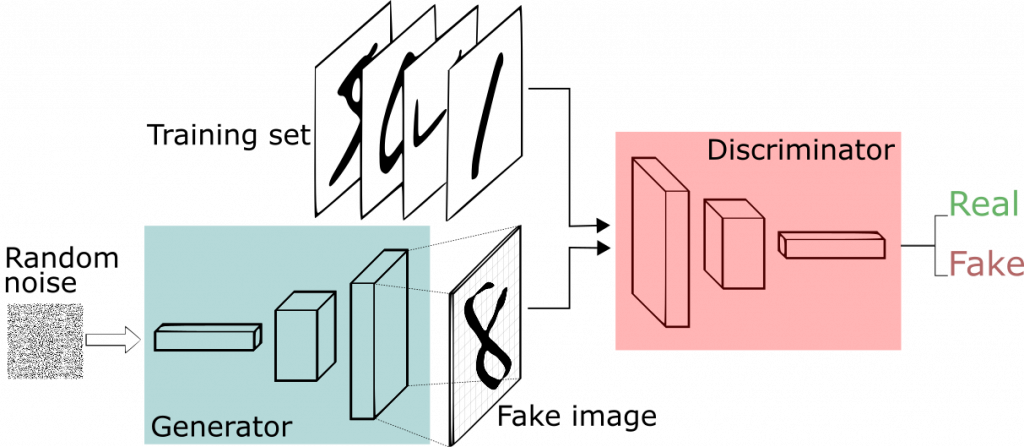
\includegraphics[width=0.9\textwidth]{images/GAN.png}
                \end{figure}
            \end{column}
        \end{columns}
      \end{frame} 

      \begin{frame}{Was ist Predictive Maintenance?}
      \begin{columns}
        \begin{column}{1\textwidth}
          Grundlegende Ziele
          \begin{itemize}
            \item Prozessüberwachung und eventuelle Steuerung \newline
            \item Vorhersagen von Maschinen/Produktionsausfällen\newline 
            \item Hilfe/Unterstüzung bei der Wartungsplanung \newline 
            \item Klassifikation von Fehlerzuständen \newline 
            \item ...
          \end{itemize}
        \end{column}
        % \begin{column}{0.4\textwidth}
        %   \begin{figure}
        %     \centering
        %      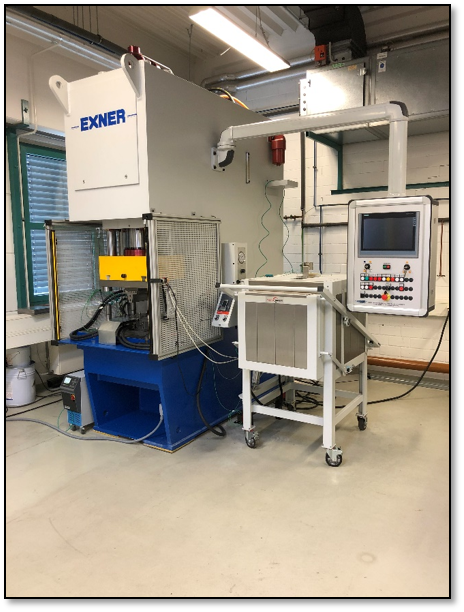
\includegraphics[width=0.6\textwidth]{images/anlage.png}
        %   \end{figure}
        % \end{column}
      \end{columns}
        \end{frame}
    

        \begin{frame}{Was ist Predictive Maintenance?}
          \begin{columns}
            \begin{column}{1\textwidth}
              \begin{itemize}
                \item PM ist als Teilbereich der Industrie 4.0 zu verstehen \newline
                \item (Nah-) Echtzeitdatenanalysen sollen Bedarfsgerechte Wartung ermöglichen \newline
                \item Großes Potential der Kosteneinsparung \newline
              \end{itemize}
            \end{column}
            % \begin{column}{0.4\textwidth}
            %   \begin{figure}
            %     \centering
            %      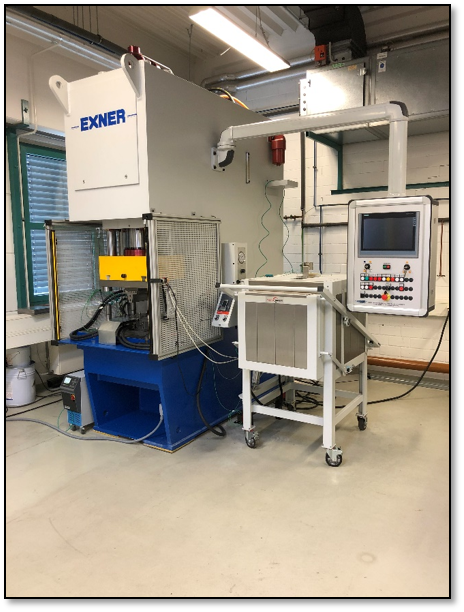
\includegraphics[width=0.6\textwidth]{images/anlage.png}
            %   \end{figure}
            % \end{column}
          \end{columns}
            \end{frame}

            \begin{frame}{Fallbeispiel: Vollautomatisierte Produktionszelle}
              \begin{columns}
                \begin{column}{1\textwidth}
                  \begin{itemize}
                    \item Automatisierungstechnik liefert Prozessdaten \newline
                    \item zusätzliche Sensorik liefert mehr Daten \newline
                    \item Ein Trend in den Daten deutet auf einen zukünftigen Fehler hin \newline
                    \item Der Fehler wird klassifiziert und eine Handlungsanweisung wird herausgegeben \newline
                    \item Der Fehler kann, bevor er größere Schäden, oder Produktionsausfälle behoben werden \newline
                    \item Wielche Schritte sind dafür Notwendig?
                  \end{itemize}
                \end{column}
                % \begin{column}{0.4\textwidth}
                %   \begin{figure}
                %     \centering
                %      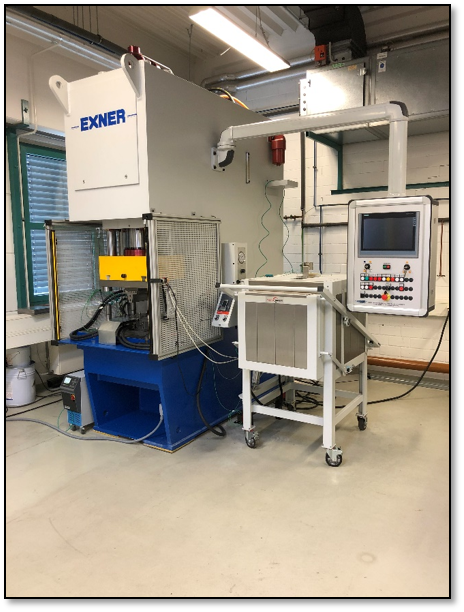
\includegraphics[width=0.6\textwidth]{images/anlage.png}
                %   \end{figure}
                % \end{column}
              \end{columns}
                \end{frame}

                \begin{frame}{Fallbeispiel: Vollautomatisierte Produktionszelle -- Outline}
                  \begin{columns}
                    \begin{column}{1\textwidth}
                      Ausgangslage Industrie 3.0
                      \begin{itemize}
                        \item Automatisierungstechnik existiert und Daten stehen der Anlagensteuerung zur Verfügung\newline
                        \item Wie werden die Daten weiterverarbeitet? Haben Sie Beispiele aus Ihrem Unternehmen? \newline
                        \item eine Möglichkeit: Auslesen der Daten über eine OPC-UA Schnittstelle \newline
                        \item Weiterleitung dieser Daten über ein schnelle und skalierbare Schnittstelle (MQTT, ApacheKafka, ...) \newline
                        \item Empfang dieser Daten auf einem Datenbankserver (MariaDB, TimeseriesDB, ApacheDruid, ...) \newline
                        \item Durchführung von Echtzeitanalysen auf einem Edge-Computer, oder in der Cloud
                      \end{itemize}
                    \end{column}
                    % \begin{column}{0.4\textwidth}
                    %   \begin{figure}
                    %     \centering
                    %      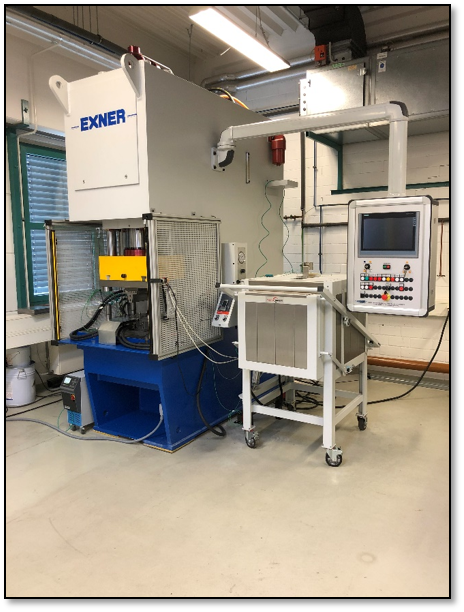
\includegraphics[width=0.6\textwidth]{images/anlage.png}
                    %   \end{figure}
                    % \end{column}
                  \end{columns}
                    \end{frame}

                    \begin{frame}{Fallbeispiel: Vollautomatisierte Produktionszelle -- Warmumformanlage}
                      \begin{columns}
                        \begin{column}{1\textwidth}
                          \begin{itemize}
                            \item Umformung und gleichzeitige Härtung von Stahl im Automobilleichtbau \newline
                            \item Probleme:
                            \item Komplexe Wirkzusammenhänge während des Prozesses \newline
                            \item Verlust von Know-How bei Standortwechseln der Produktion \newline
                            \item Langwierige Prüfverfahren zur Qualitätssicherung \rightarrow hohes Schadenspotential bei unentdeckten Fehlern \newline
                          \end{itemize}
                        \end{column}
                         \begin{column}{0.4\textwidth}
                           \begin{figure}
                             \centering
                              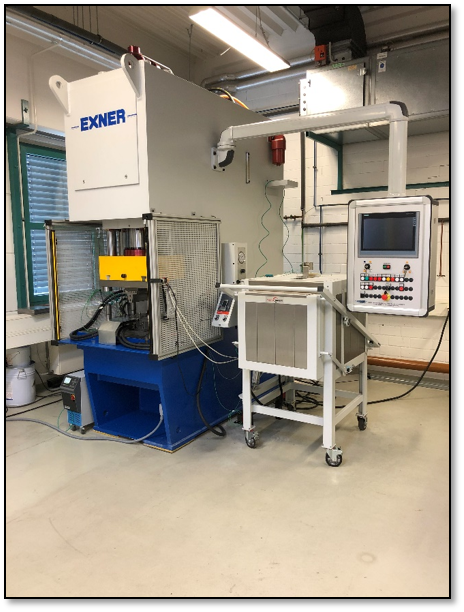
\includegraphics[width=0.6\textwidth]{images/anlage.png}
                           \end{figure}
                         \end{column}
                      \end{columns}
                        \end{frame}

                    \begin{frame}{Visualisierung eines möglichen Backends}
                      \begin{columns}
                        \begin{column}{1\textwidth}
                           \begin{figure}
                             \centering
                              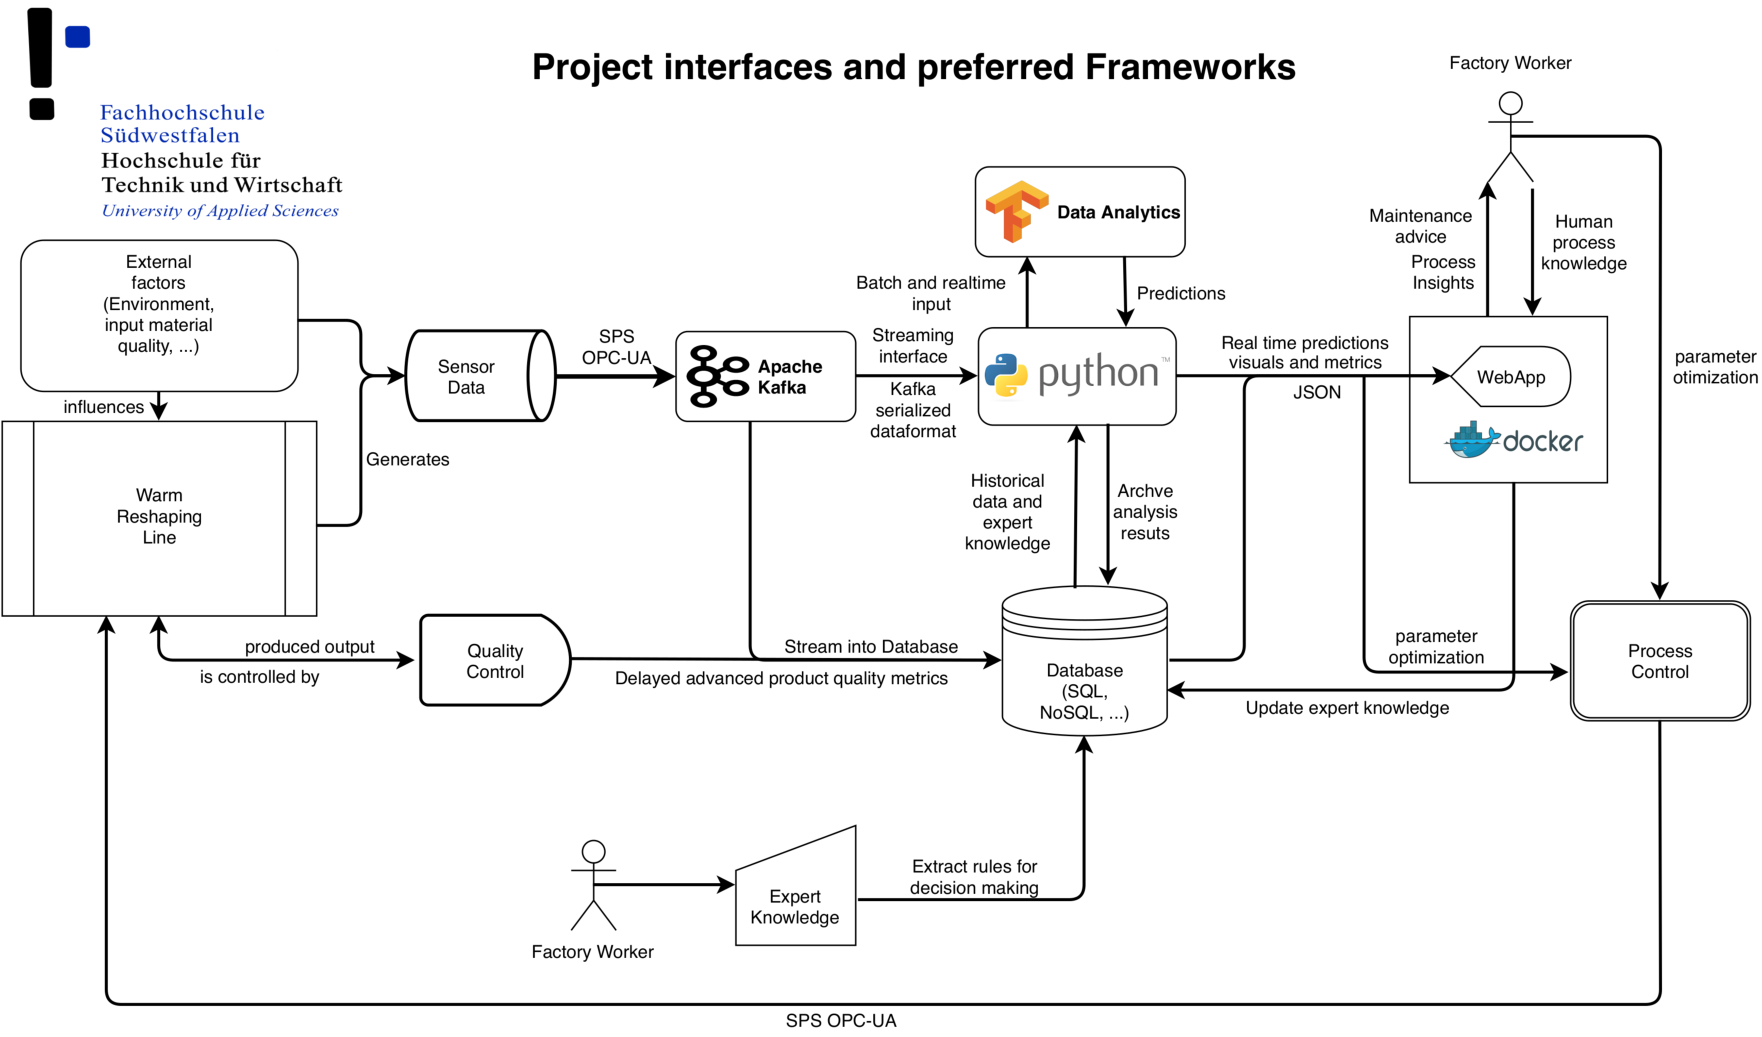
\includegraphics[width=0.6\textwidth]{images/process_v1_new.pdf}
                           \end{figure}
                         \end{column}
                      \end{columns}
                        \end{frame}

            \begin{frame}{Fallbeispiel: Vollautomatisierte Produktionszelle -- Datensammlung}
                          \begin{columns}
                            \begin{column}{1\textwidth}
                              \begin{itemize}
                                \item Prozessdaten werden mit einer OPC-UA Schnittstelle aus der übergeordneten Steuerung gelesen  \newline
                                \item Die Qualitätssicherung liefert verzögert Daten über die gefertigten Bauteile  \newline
                                \item Experten geben Know-How über den Prozess in einer strukturiterten Form einer FMEA (Failure Mode and Effects Analysis) ein \newline
                              \end{itemize}
                            \end{column}
                            % \begin{column}{0.4\textwidth}
                            %   \begin{figure}
                            %     \centering
                            %      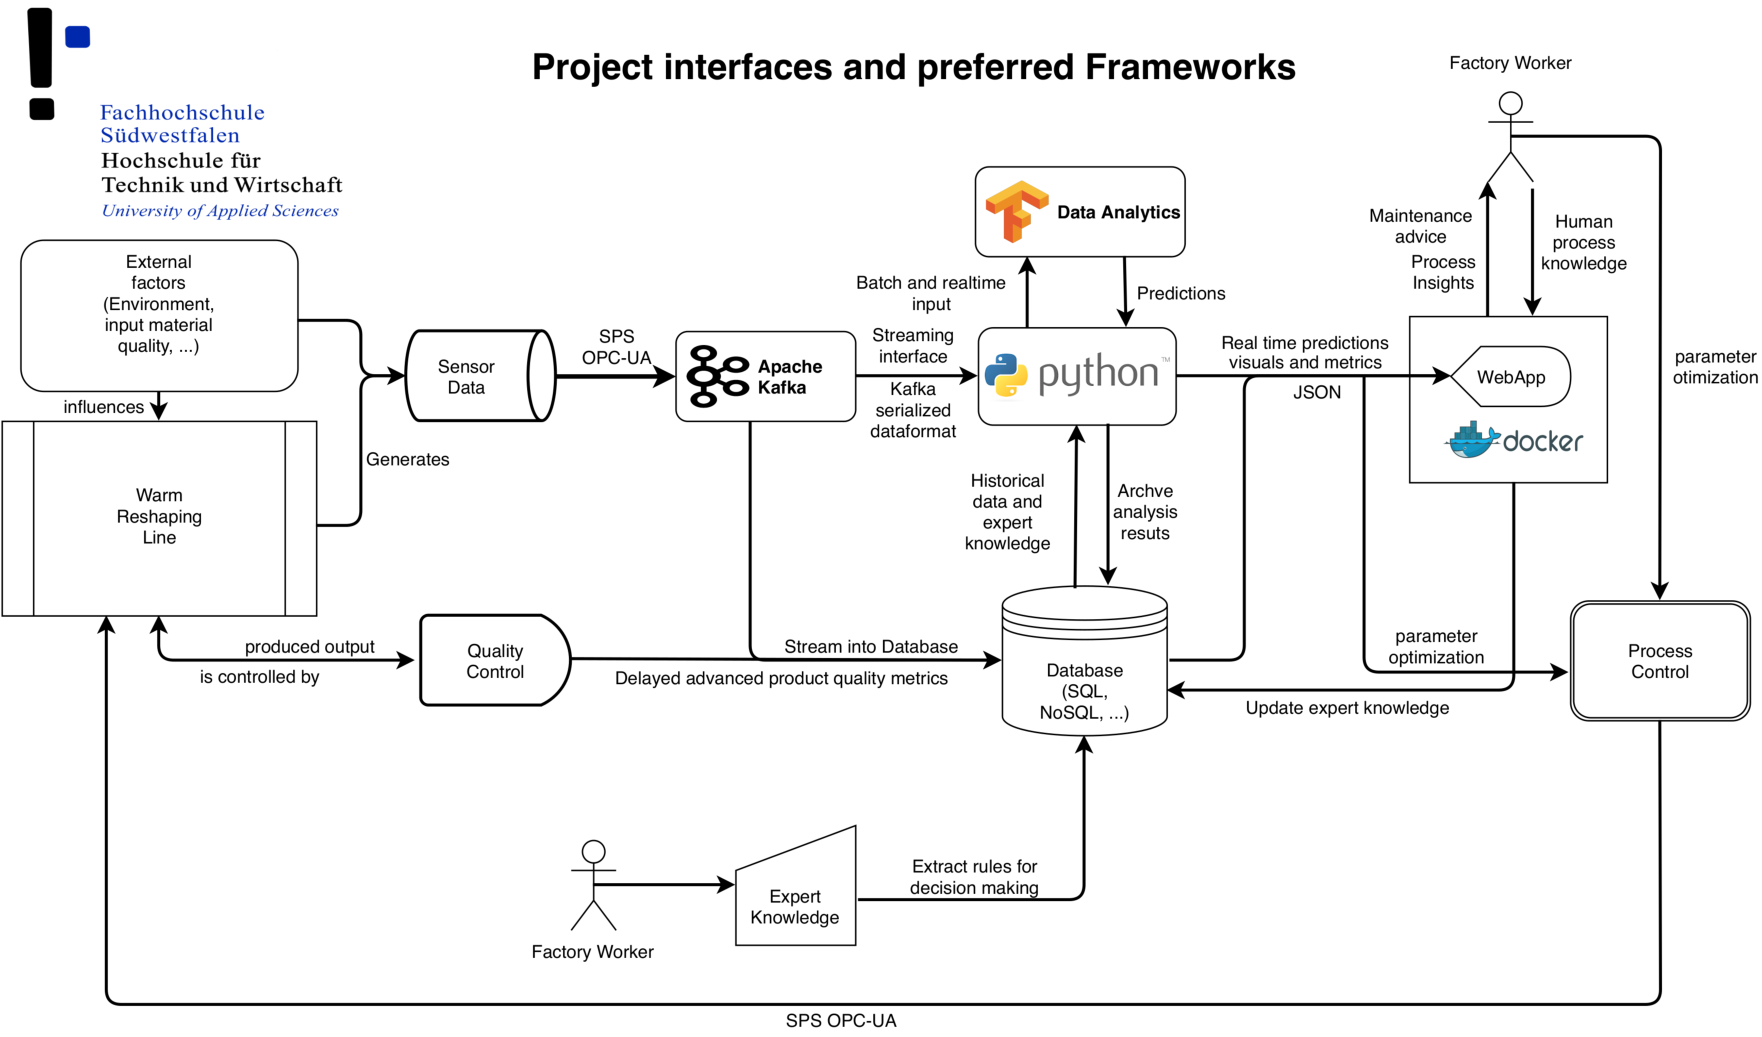
\includegraphics[width=0.4\textwidth]{images/process_v1_new.pdf}
                            %   \end{figure}
                            % \end{column}
                          \end{columns}
               \end{frame}   
          
          \begin{frame}{Fallbeispiel: Vollautomatisierte Produktionszelle -- Erste Datenverarbeitung mit einem Broker System}
                      \begin{columns}
                        \begin{column}{0.6\textwidth}
                          \begin{itemize}
                            \item Die Daten aus der Anlagensteuerung werden mit einem "Producer" an einen Broker geschickt, der den Datenstrom verwaltet \newline
                            \item Ein Brokersystem wie ApacheKafka oder MQTT kontrolliert den Datenfluss \newline
                            \item Clients können dem Broker "folgen" (subscriben) \newline
                            \item Ein sogenannter Consumer erhält diesen nun bei jedem neuen erzeugten Datenpunkt \newline
                            \item Diese Datenpunkte können dann mit einem Machine Learning Framework (sci-kit-learn, TensorFlow, PyTorch) analysiert werden \newline
                            \item Vorteil: Parallelisierung des Datenflusses möglich
                            \item Gleichzeitiges Speichern der Daten in einer Datenbank und Echtzeitverarbeitung im Datenanalyse Framework und darstellung auf einem Dashboard \newline  
                          \end{itemize}
                        \end{column}
                        % \begin{column}{0.4\textwidth}
                        %   \begin{figure}
                        %     \centering
                        %      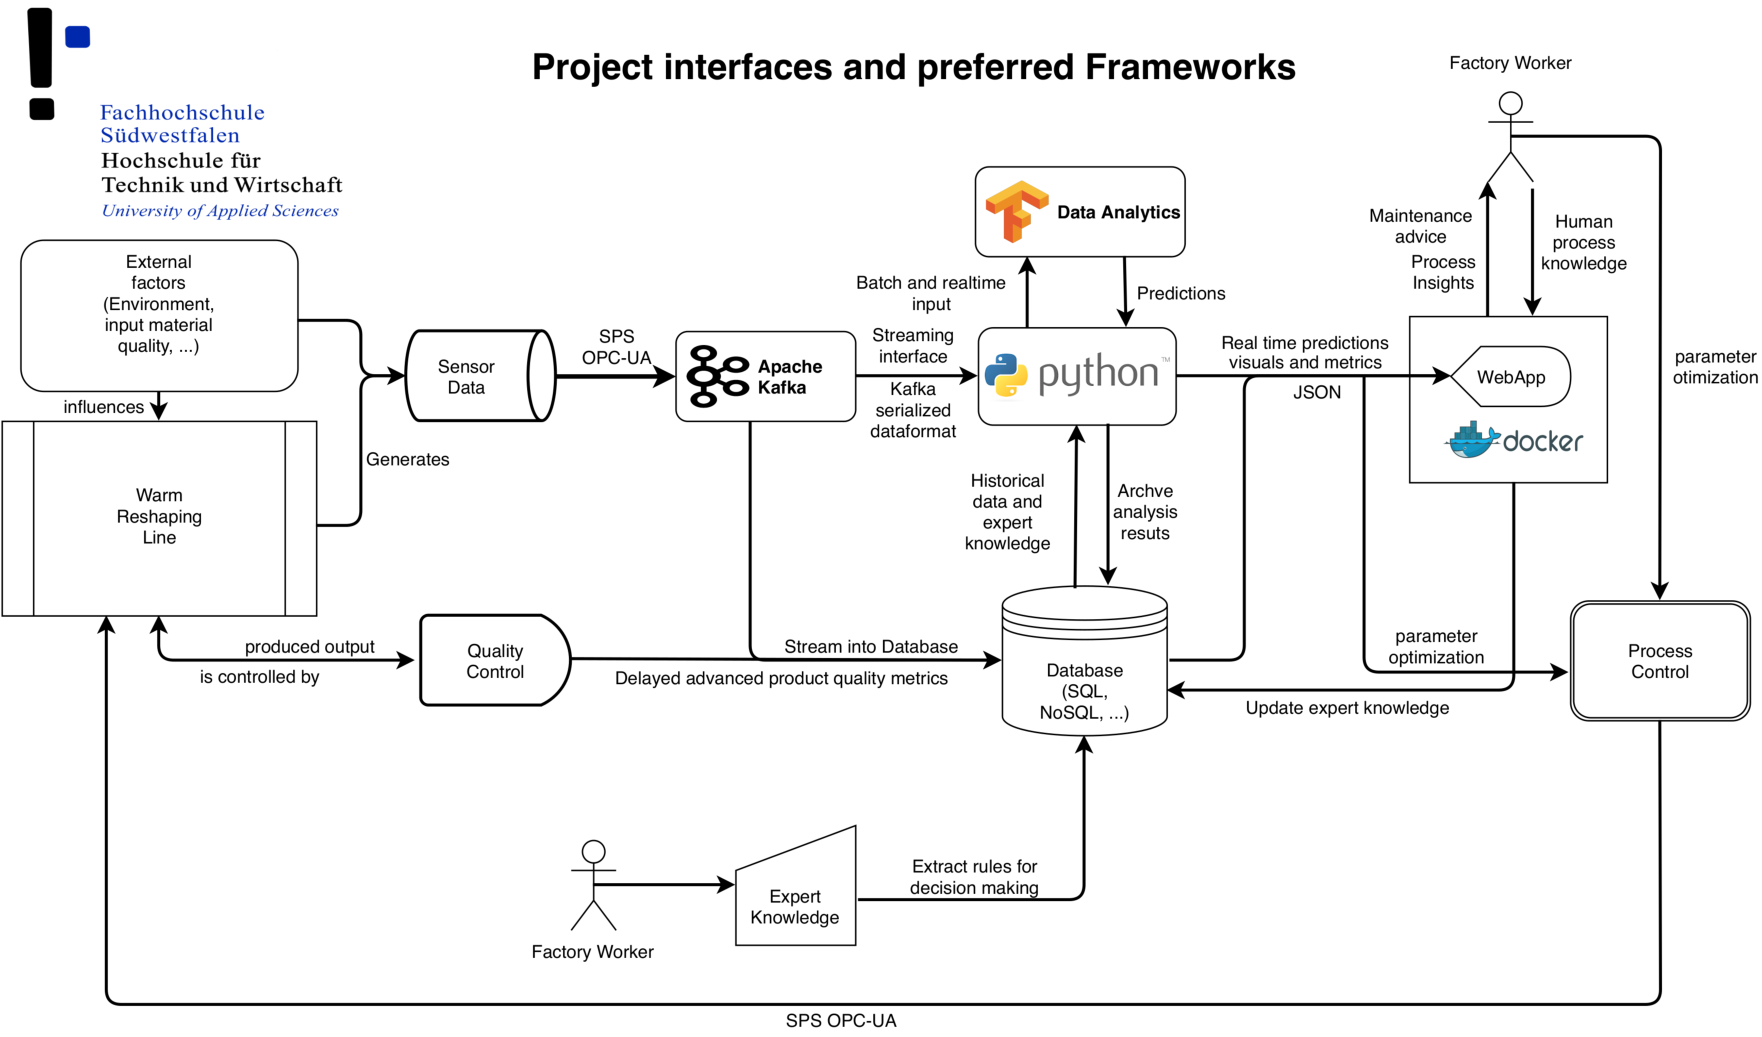
\includegraphics[width=0.4\textwidth]{images/process_v1_new.pdf}
                        %   \end{figure}
                        % \end{column}
                      \end{columns}
           \end{frame}

           \begin{frame}{Fallbeispiel: Vollautomatisierte Produktionszelle -- Darstellung der Daten für einen Maschinenoperator}
            \begin{columns}
              \begin{column}{0.6\textwidth}
                \begin{itemize}
                  \item Eine vereinfachte visuelle Darstellung der Maschinenparameter kann z.B. in einem Dashboard ausgegeben werden \newline
                  \item Erfahrene Operatoren können aus diesen Daten und ersten Analysen Schlussfolgerungen ziehen \newline
                  \item mögliche Parameteranpassungen im Prozess können durch diesen Operator durchgeführt werden
                \end{itemize}
              \end{column}
               % \begin{column}{0.4\textwidth}
               %   \begin{figure}
               %     \centering
               %      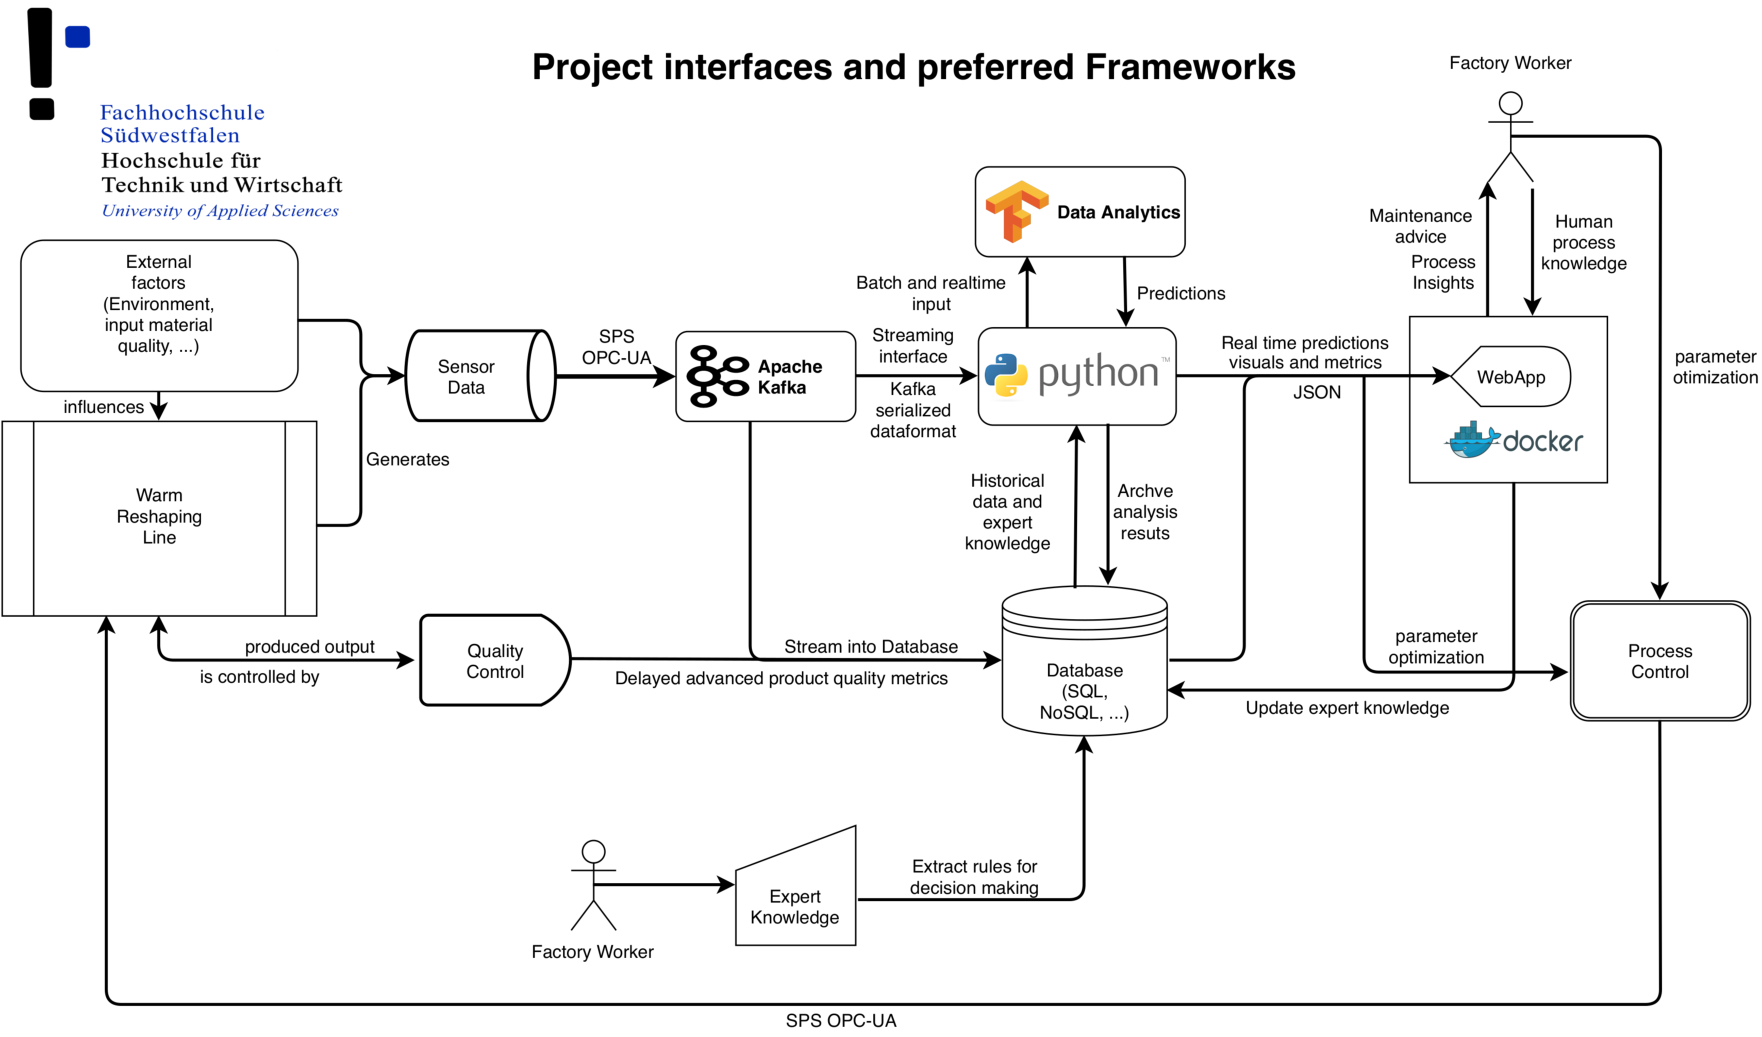
\includegraphics[width=0.4\textwidth]{images/process_v1_new.pdf}
               %   \end{figure}
              %  \end{column}
            \end{columns}
          \end{frame}

          \begin{frame}{Fallbeispiel: Vollautomatisierte Produktionszelle -- Direkte Handlungsanweisungen an einen Operator}
            \begin{columns}
              \begin{column}{0.6\textwidth}
                \begin{itemize}
                  \item Vorhersagen des trainierten Machine Learning Modells werden mit einer FMEA abgeglichen \newline
                  \item eine FMEA enthält die häufigsten Fehler und Defekte einer Analage \newline
                  \item Problemlösungen werden hier strukturiert skizziert \newline
                  \item unerfahrene Operatoren können hier durch das gesammelte Expertenwissen Entscheidungen treffen\newline
                  \item Operatoren können für den Vorhergesagten Zeitpunkt Mechaniker zur Wartung der Maschine anfordern
                \end{itemize}
              \end{column}
               % \begin{column}{0.4\textwidth}
               %   \begin{figure}
               %     \centering
               %      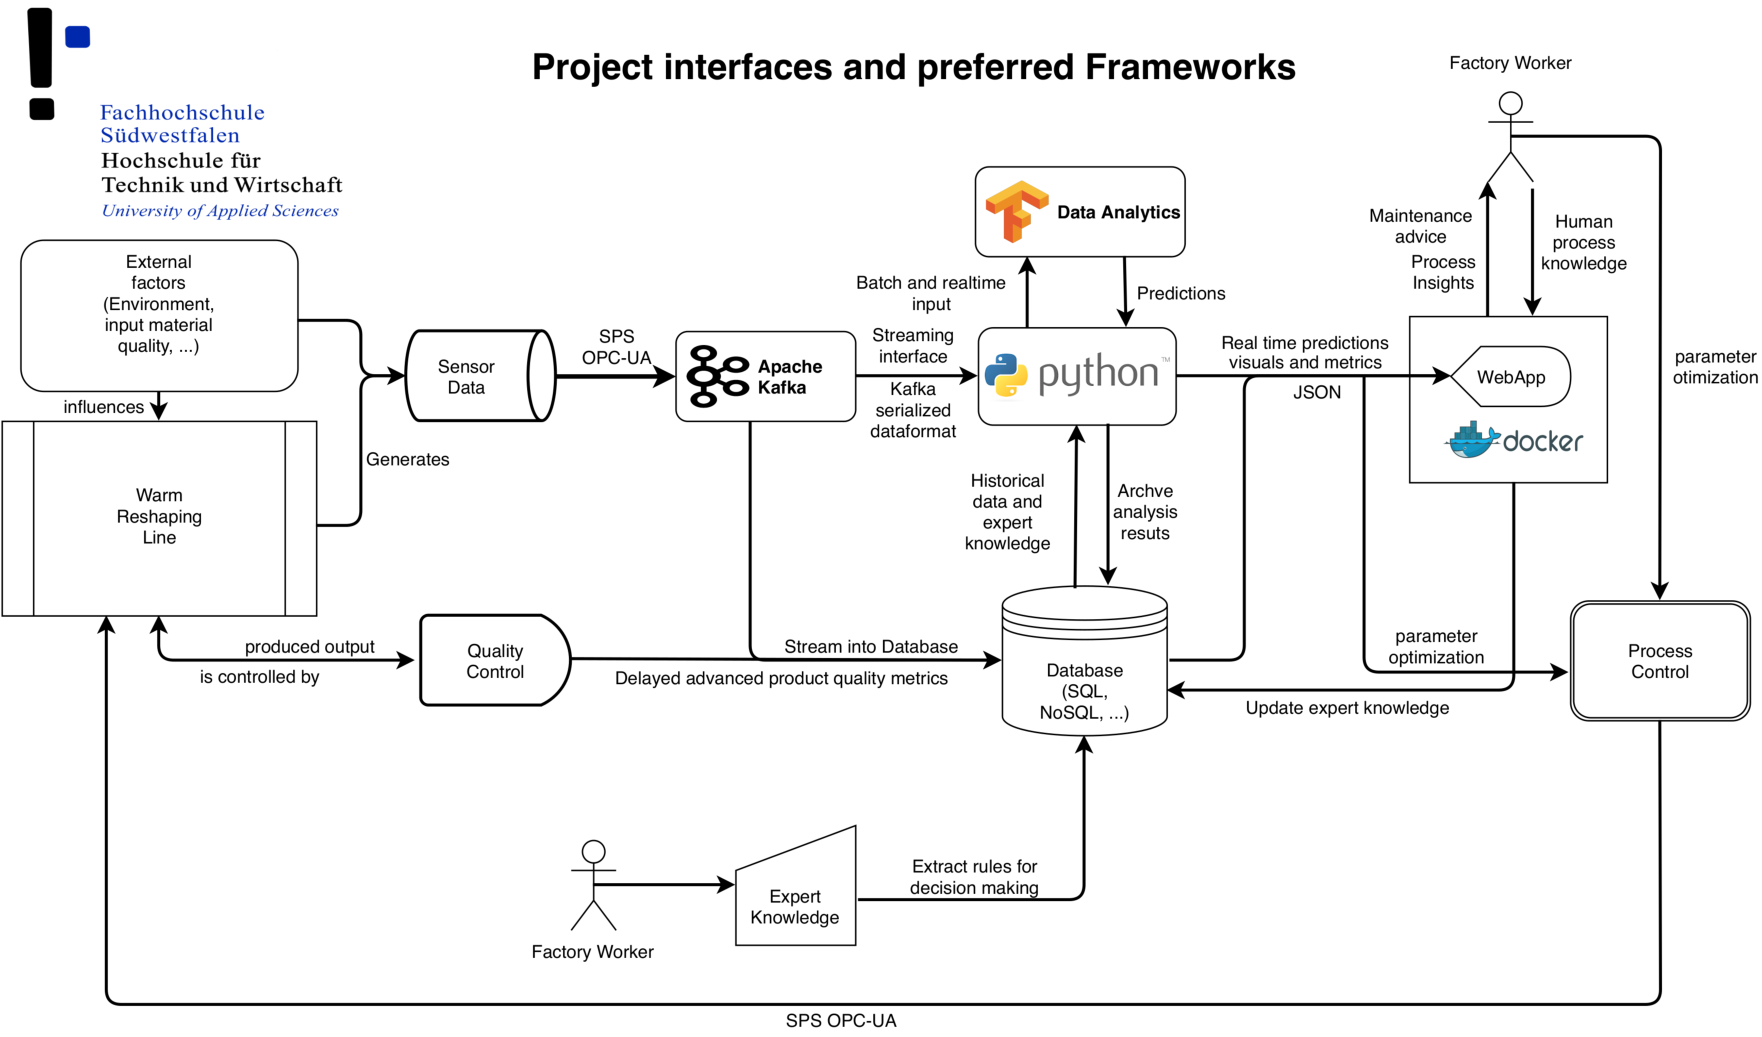
\includegraphics[width=0.4\textwidth]{images/process_v1_new.pdf}
               %   \end{figure}
              %  \end{column}
            \end{columns}
          \end{frame}


          \begin{frame}{Fallbeispiel: Vollautomatisierte Produktionszelle -- Direkte Handlungsanweisungen an die Prozessteuerung (Dangerzone)}
            \begin{columns}
              \begin{column}{0.6\textwidth}
                \begin{itemize}
                  \item Mögliche kritische Zustände können direkt zu einem Stop der Produktion führen \newline
                  \item Anpassung der Prozessparameter direkt durch die Software \rightarrow vollständig autonomes System \newline 
                  \item Mensch wird nur noch zum Eintragen von Know-How benötigt \newline
                \end{itemize}
              \end{column}
               % \begin{column}{0.4\textwidth}
               %   \begin{figure}
               %     \centering
               %      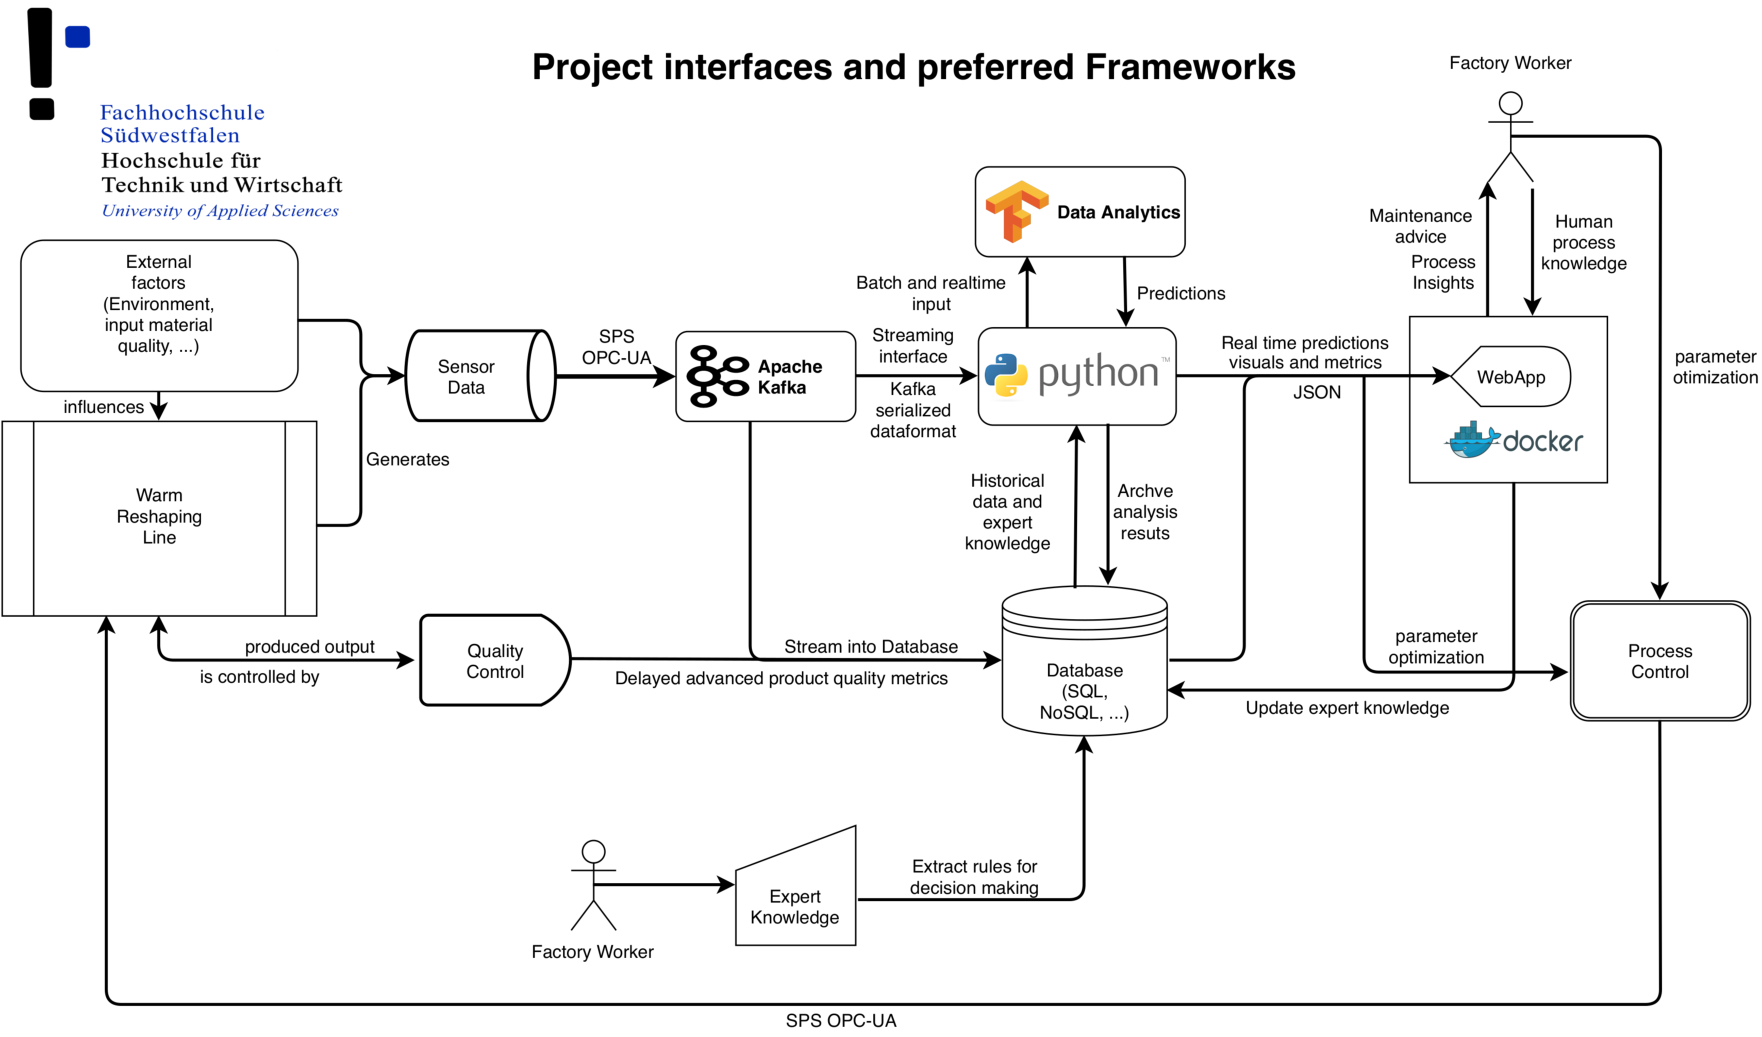
\includegraphics[width=0.4\textwidth]{images/process_v1_new.pdf}
               %   \end{figure}
              %  \end{column}
            \end{columns}
          \end{frame}

          
          \begin{frame}{Andere Beispiele: Wo ist PM finanziell besonders sinnvoll?}
            \begin{columns}
              \begin{column}{1\textwidth}
                \begin{itemize}
                  \item Kraftfahrzeuge: Sensorik in Verschleißteilen kann Totalausfälle vermeiden \newline
                  \item Luftfahrt: Der Ausfall von Passagier- oder Luftfrachtflügen kann mit guten Ausfallvorhersagen verhindert werden   \newline 
                  \item Schinenverkehr \newline
                \end{itemize}
              \end{column}
               % \begin{column}{0.4\textwidth}
               %   \begin{figure}
               %     \centering
               %      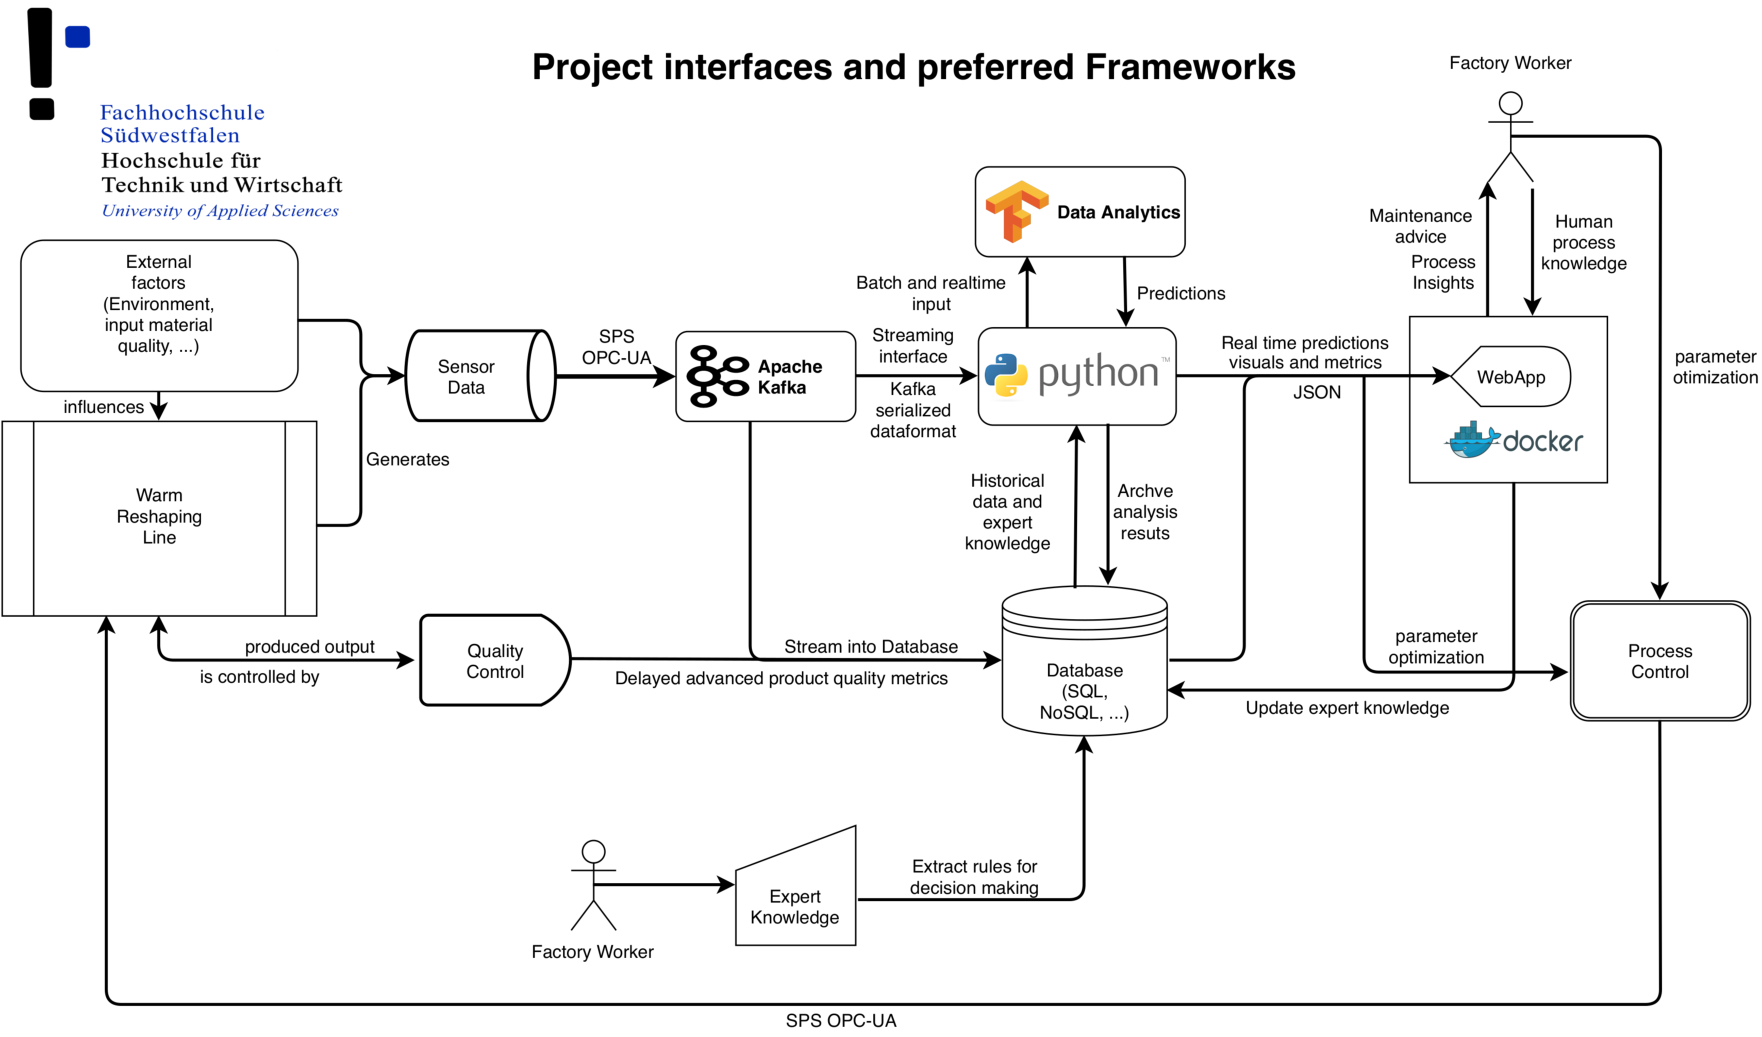
\includegraphics[width=0.4\textwidth]{images/process_v1_new.pdf}
               %   \end{figure}
               % \end{column}
            \end{columns}
          \end{frame}

% \begin{frame}{Experimental Setup -- What is the underlying process?}
%   \begin{columns}
%     \begin{column}{1\textwidth}
%     Process description
%       \begin{itemize}
%         \item Heating metal sheet to target temperature
%         \item Transfer to a hydraulic press
%         \item Reshaping the metal sheet while hot 
%         \item Cool down while in contact with cool surface using the correct cooling rate
%         \item Transfer to further manufacturing
%       \end{itemize}
%     \end{column}
%     \begin{column}{0\textwidth}
%    % \begin{figure}
%    % \centering
%    %             \includegraphics[width=0.9\textwidth]{images/intro/intro.pdf}
%    % \end{figure}
%     \end{column}
%   \end{columns}
% \end{frame}


% \begin{frame}{Experimental Setup -- What is the underlying process?}
%   \begin{center}
%    \smartdiagramset{border color=fhblue,
%    set color list={fhblue!35!white, fhblue!20!white, fhblue!20!white, fhblue!20!white, fhblue!20!white}}
%    \smartdiagram[sequence diagram]{Heating,
%    Transfer, Reshaping, Cooling, Manufacturing}
%   \end{center}
%   Heating metal sheet to target temperature
% \end{frame}
% 
% \begin{frame}[noframenumbering]{Experimental Setup -- What is the underlying process?}
%   \begin{center}
%     \smartdiagramset{border color=fhblue,set color list={fhblue!20!white, fhblue!35!white, fhblue!20!white, fhblue!20!white, fhblue!20!white}}
%     \smartdiagram[sequence diagram]{Heating,Transfer, Reshaping, Cooling, Manufacturing}
%   \end{center}
%   Transfer heated metal sheet into hydraulic press
% \end{frame}
% \begin{frame}[noframenumbering]{Experimental Setup -- What is the underlying process?}
%   \begin{center}
%   \smartdiagramset{border color=fhblue,set color list={fhblue!20!white, fhblue!20!white, fhblue!35!white, fhblue!20!white, fhblue!20!white}}
%   \smartdiagram[sequence diagram]{Heating,Transfer, Reshaping, Cooling, Manufacturing}
%   \end{center}
%    Reshaping of metal sheet while it's hot 
% \end{frame}
% 
% \begin{frame}[noframenumbering]{Experimental Setup -- What is the underlying process?}
%   \begin{center}
%     \smartdiagramset{border color=fhblue,  set color list={fhblue!20!white, fhblue!20!white, fhblue!20!white, fhblue!35!white, fhblue!20!white}}
%     \smartdiagram[sequence diagram]{Heating,  Transfer, Reshaping, Cooling, Manufacturing}
%   \end{center}
%   Cool down while in contact with coole surface with correct cooling rate 
% \end{frame}
% 
% \begin{frame}[noframenumbering]{Experimental Setup -- What is the underlying process?}
%   \begin{center}
%     \smartdiagramset{border color=fhblue, set color list={fhblue!20!white, fhblue!20!white, fhblue!20!white, fhblue!20!white, fhblue!35!white}}
%      \smartdiagram[sequence diagram]{Heating,     Transfer, Reshaping, Cooling, Manufacturing}
%   \end{center}
%   Transferring metal sheet to further manufacturing
% \end{frame}
%     
% % \begin{frame}{Development of the demonstration plant -- Why build one on our own?}
% % \begin{columns}
% %   \begin{column}{1\textwidth}
% %     \begin{itemize}
% % 
% %       \item Sensors
% %       \begin{itemize}
% %         \item[\rightarrow] Possible sensors for later implementation in production plants
% %         \item[\rightarrow] Temperature monitoring with infrared cameras
% %         \item[\rightarrow] Temperature Sensors in the stamp
% %       \end{itemize}
%       \item Implementation of a completely automonous system 
%       \begin{itemize}
%         \item[\rightarrow] Edge computing on site
%         \item[\rightarrow] Backend development\newline
%       \end{itemize}
%       
%       %mit bildern/video
%     \end{itemize}
%   \end{column}
%   \begin{column}{0.6\textwidth}
%  % \begin{figure}
%  %  \centering
%  %  \includegraphics[width=0.9\textwidth]{images/intro/intro.pdf}
%  % \end{figure}
%   \end{column}
% \end{columns}
% \end{frame}




\begin{frame}[allowframebreaks]{References}
 \bibliographystyle{ieeetr}
 \bibliography{lit.bib}
\end{frame}
\end{document}
